\documentclass[]{report}
\usepackage[utf8]{inputenc}
\usepackage{amsmath,fullpage,amsfonts,amssymb,tikz,geometry,amsthm,pgfplots,relsize,graphicx}
\usepackage[boxruled]{algorithm2e}
\geometry{margin=0.5in}
\usetikzlibrary{matrix}
\pgfplotsset{soldot/.style={color=blue,only marks,mark=*}} \pgfplotsset{holdot/.style={color=blue,fill=white,only marks,mark=*}}
\usepackage{hyperref}
\usepackage{setspace}
\doublespacing
\title{Scaling MCMC methods for Bayesian neural networks}
\author{Yiu Sing Lau}
\date{}
\begin{document}

\maketitle

\renewcommand{\abstractname}{ACKNOWLEDGEMENTS}
\begin{abstract}
Thank you very much

\end{abstract}

\renewcommand{\abstractname}{ABSTRACT}

\begin{abstract}
Neural network models have seen tremendous success in predictive tasks in machine learning and artificial intelligence(quote), with some attributing their success to the use bayesian inference \cite{mandt2017stochastic}. STAN is a state of the art software for Bayesian statistical computing used mainly in the statistical community, however, it is not optimzed for use with neural network models. In this thesis, we replicated much of STAN's No U-Turn sampler in PyTorch and explore its use for sampling from bayesian neural network models. We were able to explore different samplers,model structures and their sampling and predictive performances, on a benchmark classification task. We found that bayesian inference improves predictive performance in general but care is needed with the choice of prior and MCMC sampler. 

\end{abstract}
\tableofcontents 

\chapter{Introduction}
\section{STAN}

STAN has replaced most Bayesian statistical softwares like JAGS and WINBUGS as the recommended tool for Bayesian inference requiring Markov Chain Monte Carlo (MCMC)  because of its effectiveness, relative ease to learn, clear and extensive documentation, as well as its large community of users and expert support staff. Roughly based on the NUTS sampler, it has since evolved from the original NUTS sampler and has many more features built in to facilitate sampling and diagnosing sampling issues.

In Chapter 2, after giving a short introduction to MCMC, we will give an overview of Hamiltonian Monte Carlo, which the foundation on which NUTS is built. Then we will explain the version of No U-TURN sampler (NUTS) implemented in STAN, highlighting its difference from the original implemnted in \cite{hoffman2014no}. Adaptive tuning strategies for the step size parameter and covariance metric will also be discussed. Termination criteria for the NUTS sampler will be discussed. The exhasutive terminal criteiron for NUTS (XHMC) , which has not been exposed in the latest version of STAN yet, has been shown to improve sampling efficiency in correlated distributions.  \cite{betancourt2016identifying}. Experiments comparing its performance against the default termination criterion will be discussed in chapter 4. Finally, we discuss some of the numerical tricks used by STAN that are omitted in the official documentation but can be critical for creating a robust implementation. 





\section{Bayesian Neural Network }

Neural network models has become hugely popular under the name of deep learning, attracting a lof of attention from researchers and practitioners alike. Many of its successes come from applications to problems in vision, text, speech, and many other sub-fields in the field of Artificial Intelligence. 


In Chapter 3 we give a brief overview of the Bayesian neural network literature and identify areas where we feel could benefit from new developments in NUTS and related sampling techniques. In Neal's and Cho's work, sampling from the posterior distribution was done by alternating between the lower and higher level parameters in a block-Gibbs fashion. With the model and data they used, they found that joint sampling offered no improvement over Gibbs sampling for sampling the hyperparameter. We found that NUTS is capable of sampling the hyperparameter quite well, is more robust to tuning parameters, and requires much less manual tuning. 

Then we talk about the choice of prior for neural network models. Originally it was standard to put a hierarchical prior on the model weights, but in the new wave of Bayesian deep learning literature the standard normal prior is used most of the times. Recently shrinkage priors like the horseshoe prior have been used to automatically regularize the weights. In the paper the authors used variational inference which might miss important features of the posterior distribution. We compared a range of priors, including the shrinkage prior, and found that the standard normal prior performed best in terms of both effective sample size and predictive accuracy. 

While the use of shrinkage priors should eliminate much of the need for model selection: one would simply fit the largest model possible and let the shrinkage prior eliminate any excessive capacity, in practice sampling from such a model might prove too difficult, for example having too many hidden layers might result in vanishing or exploding gradients(quote). There are also tuning parameters, like the activation function, which can not be chose by shrinkage priors. This necessitates model selection techniques. Model selection by information criterion like AIC and BIC is not backed by theory because neural networks violate one of their regularity conditions, namely that the model must have non-singular Fisher matrix. The Watanabe Information Criterion (WAIC) is designed to overcome this problem for all singular models. We experimented with the WAIC but found that it failed to choose the model that minimizes the test error on the dataset we chose. 

We also experimented with Stochastic Gradient Hamiltonian Monte Carlo (SGHMC), a version of Hamiltonian Monte Carlo that only uses a fraction of the data to approximate the gradient of the full posterior density function. In \cite{betancourt2015fundamental} the author showed that stochastic gradients causes divergence in high dimensional problems and is not recommended. Our experimentation shows that SGHMC can yield better predictive performance than full HMC but it requires careful tuning and is not robust to the initial tuning parameters. 

Initialization strategies where the weights are sampled from the normal distribution whose variance is scaled by the number of incoming units have been widely adopted for improving the final predictive accuracy. It motivates one to use such scaled normal distributions as the prior distribution. Its impact on predictive accuracy and sampling quality will be discussed in Chapter 4. 

Finally, we explore the use of NUTS for sampling from bayesian neural networks.

Model selection in the neural network literature is usually done by choosing the model that minimizes the error on a validation set. This works well for the problems 







Currently the literature is dominated by frequentist methods where a local optimum of the loss function is found by stochastic optimization. 

Talk about research by McKay and Neal.




\chapter{STAN}
\section{Hamiltonian Monte Carlo}

Bayesian Inference can be simply summarized by the specification of a likelihood and a prior function. Suppose $\theta \in \mathbb{R}^d$ is the parameter of the likelihood function for observed data $X \sim p(x| \theta)$, we can
model our uncertainty about it with a prior function $p(\theta)$. Upon observing the data, we can perform Bayesian inference by using information from the posterior distribution 

\[ p(\theta | x ) \propto p(x | \theta) p(\theta) \]

Examples: MAP, marginal posterior estimation, credible intervals. The exact calculation of the normalizing constant $Z = \int p(x | \theta) p(\theta) d\theta $ is possible for certain convenient functions only, and we must rely on Markov Chain Monte Carlo (MCMC) to calculate posterior quantities. The most basic form of MCMC is the Metropolis-Hastings sampler. 


Suppose we have a an unnormalized density $p(x)$, and $q(x,y)$ is a proposal function such that conditional on the current state $x$, the probability of moving from $x$ to a measurable set $A$ is denoted by $q(x,A)$, we can calculate the Hastings ratio
\[ r(x,y) = \frac{p(y)q(y,x)}{p(x)q(x,y)}. \]

Then we accept the move to state $y$ with probability $ \min (1, r(x,y)) $, and stay in the current state otherwise.

\begin{algorithm}
\caption{Metropolis Hastings Sampler}
\KwIn{$x_0$ initial state, $p(\cdot)$ unnormalized target density, $q(\cdot,\cdot)$ proposal density}


\For{$i = 1:n$}{
  	Draw $x_{prop}$ from $q(x_{i-1},\cdot)$ \;  	
  	Accept $x_{prop}$ with probability $\min(1,r(x_{prop},x_{i-1}))$ \;
  	
}
 
 
\end{algorithm}


The choice of a proposal distribution is highly critical to the efficiency of the MH sampler. Even after a proposal distribution is chosen, there is usually further tuning parameters that needs to be chosen. The acceptance probability is an important quantity which 
can be optimized . In the case of a target distribution with zero correlation between components and using a symmetric gaussian proposal, the optimal acceptance rate is 0.234.\cite{roberts1997weak,gelman1996efficient,roberts2001optimal} 

Very much like optimization \cite{wright1999numerical}, for differentiable density
functions, information about the gradient can be useful for proposing the next
state, which brings us to the subject of Hamiltonian Monte Carlo.


The use of MCMC in statistical applications began with \cite{geman1984stochastic,besag1986statistical} in the field of image analysis. Because of the high-dimensional nature of image datasets, initially only the Gibbs sampler were used, circumventing the well known slow-mixing/low-acceptance behaviour of the random-walk Metropolis-Hastings sampler in high dimensions. The introduction of Hamiltonian Monte Carlo into the field of statistics by Neal \cite{neal2011mcmc,neal2012bayesian}, who built on the work of physicists using HMC to simulate from lattice field models \cite{duane1987hybrid}, brings an exciting new tool that allows statisicians to simulate much more efficiently from high-dimenisonal distributions. Unfortunately, because of the relative difficulty in implementing such samplers its use in statistics has been limited. In the last few years there has been a rebirth of the HMC sampler, with new developments that try to utilize information about the local curvature of the density function during  sampling \cite{girolami2011riemann,betancourt2013general}, as well as  automate the selection of tuning parameters.  \cite{hoffman2014no,betancourt2016identifying}. 
Arguably the most important development that is part of this rebirth is the development of the No U-Turn Sampler and the STAN software which uses NUTS as its main sampler. We  also have a better theoretical understanding of the HMC with work (cite)
that provides a differential geometric interpretation of the sampler and conditions under which geometric convergence can be obtained.

First we give a brief introduction to the HMC,explaining its algorithm and listing its major features and advantages. 

Suppose we have a density $p(x),x \in \mathbb{R}^d$ from which we would like to
sample. If $p(x)$ is simply the marginal density of some distribution $p(x,y),
(x,y) \in \mathbb{R}^{d+p}$ in a larger space containing the original domain, then sampling from $p(x,y)$ and keeping only the $x$'s is equivalent to sampling from $p(x)$ directly. These extra variables introduced are called auxillary variables. The auxillary variables methods are known to speed up sampling by introducing extra degrees of freedom in the state space and allows the chain to move more easily across different parts of it. The Swendsen-Wang sampler \cite{wang1990cluster}, the slice sampler\cite{wang1990cluster} are well known examples of this class of methods. See \cite{liang2011advanced,liu2008monte} for more details.

The Metropolis-Hastings sampler as introduced above is a general algorithm that allows us to sample from any distribution, discrete, continuous or neither, as long as we know its density up to its normalizing constant. The Hamiltonian Monte Carlo (HMC) sampler is a particular class requires the unnormalized density be continuous and differentiable. 


We denote the unnormalized density of the target distribution by $\pi(q)$, and the normalizing constant by $Z = \int\pi(q)dq $, and we define the potential energy function $V(q)$ as 
\[ V(q) =  -\log \pi(q) \]
If we now introduce a kinetic energy function $T(p)$, and define
the Hamiltonian as the total energy, i.e., sum of the kinetic and potential energy functions, 

\[ H(q,p) = V(q) + T(p) \]

we get that 

\[\pi(q,p) \propto  \exp(-H(q,p)) \]

has $P(q)$ as the marginal density, and thus defines an auxiliary variable method. In statistical applications,we usually have $P(x)$ as the unnormalized posterior
density, 
\[U(q) = -\log(\text{prior}(q) \cdot \text{likelihood}(q|data) ), \]
and 
\[T(p) = \sum_{i=1}^d \frac{p_i^2}{m_i} \]
,which is equivalent to introducing an independent multivariate Gaussian random variable of
the same dimension as the original distribution as an auxiliary variable. 

Note that there is physical interpretation of the system. The Hamiltonian uniquely determines the motion of a particle, whose position in space at any time is described by the $q$ coordinates, and whose momentum is described by the $p$ coordinates. Its motion can be described by solving a system of ordinary differential equations in Hamiltonian dynamics, known as Hamilton's equations:
\begin{align}
    \frac{dq}{dt} &= \frac{\partial H}{\partial p } \\
    \frac{dp}{dt} &= -\frac{\partial H}{\partial q}
\end{align}



To simulate the trajectory of a particle given its initial state $(q_0,p_0)$ one
would have to solve Hamilton's equations. Unfortunately, there are in general no
explicit solutions for Hamilton's equations except for trivial models. One would
then have to resort to numerical methods that discretize the Hamiltonian
dynamics \cite{leimkuhler2004simulating}. The discretization should
possess some nice properties , including reversibility and volume-preservation, to ensure convergence to the target distribution, as well as  maintain 
stability and accuracy of the approximation over long trajectories, the lack of which significantly reduces the efficiency of the sampler, irrespective of model-related factors which might affect sampling efficiency, like parametrization or posterior correlation.  

For the simple version of HMC where the momentum variable is independent from the position variable, i.e. $\pi(p|q)=\pi(p)$, an easy-to-implement integrator which is both volume-preserving and reversible, with lower approximation error than conventional alternatives for numerically solving like Euler's method, known as the leapforg integrator, exists and works as follows. At time $t$ of the trajectory, given its current position and momentum, $q(t)$ and $p(t)$,and step size $\epsilon$, we would update the position and momentum at time $t+\epsilon$ by setting 

\begin{align}
    &p(t+\frac{\epsilon}{2}) = p(t) - \frac{\epsilon}{2}\cdot \frac{\partial
    U}{\partial
    q}q(t) \\
    &q(t+\epsilon) = q(t) + \epsilon  \frac{\partial K}{\partial p}(p(t+\epsilon/2))
    \\
    &p(t+\epsilon) = p(t + \frac{\epsilon}{2}) - \frac{\epsilon} {2} \cdot \frac{\partial U}{\partial
    q}(q(t+\epsilon))
\end{align}

One leapfrog step consists of first a half-step update for momentum, a full-step
for position, then another half-step for momentum. Since the update for momentum
at time $t+\epsilon$ and time $t+\epsilon + \frac{\epsilon}{2}$ both involve
$q(t+\epsilon)$, when $L$ leapfrog steps are used performed sequentially with
 stepsize $\epsilon$, as done during the simulation of a trajectory when proposing a new
 state,  we can combine the updates in the implementation, so that instead of perform two half steps for momentum $p(t+\frac{\epsilon}{2}) \rightarrow p(t+\epsilon)$, then $ p(t+\epsilon) \rightarrow p(t+\epsilon + \frac{\epsilon}{2})$, we can perform a full step for momentum $p(t+\frac{\epsilon}{2}) \rightarrow p(t+ \epsilon + \frac{\epsilon}{2}) $ as 
\begin{align}
p(t+\epsilon + \frac{\epsilon}{2})  
&= p(t+\epsilon) - \frac{\epsilon}{2} \frac{\partial U}{\partial q }(q(t+\epsilon)) \\
&= p(t+\frac{\epsilon}{2}) - \frac{\epsilon}{2} \frac{\partial U}{\partial q }(q(t+\epsilon)) - \frac{\epsilon}{2} \frac{\partial U}{\partial q }(q(t+\epsilon)) \\
&= p(t+\frac{\epsilon}{2}) - \epsilon \frac{\partial U}{\partial q }(q(t+\epsilon))
\end{align}

Note, however, we still need $p(t+\frac{\epsilon}{2})$ to perform the full
steps, so that at least one half step has to be made for the momentum. Also, in
this alternative implementation of the leapfrog integrator, momentum $p$ is
always one half step ahead of position, hence the last update for momentum has
to be a half step so we end up with $p(t+\epsilon L)$ and $q(t+\epsilon L )$,
both synchronized. The two implementations yield exactly the same updates, bar
loss of accuracy from calculating the sums and extra computer time for updating
the momentum variables twice in the naive implementation. 

Starting at some initial time $t_0$, with initial coordinates $(q(t_0),p(t_0))$, the position and momentum at time $t+s$ can be determined by repeating the steps above roughly $\frac{s}{\epsilon} = L$ times, taking care to round up or down. 

One advantage of the leapfrog integrator over other more well-known methods for
solving ODE numerically such as Euler's method is that it is symplectic, which
means it preserves volume in the phase space, just like the Hamilonian. This
contributes to its relative stability along the trajectory compared to Euler's
method and its modifications. An unstable trajectory as simulated by Euler's
method would propose a state that has diverged from the energy level set to
which the intitial state belong, which makes proposals much more likely to be
rejected, especially in high dimensional distributions.  However,
the leapfrog method does not preserve the Hamiltonian, so the energy of the particle would
oscillate as it is being simulated. It has important implications for the
sampling algorithm. Intuitively, this breaks the law of conservation of energy
and suggests the position of the particle at the end of its trajectory may
deviate from the correct trajectory, on which the energy should be preserved.
Reducing the stepsize would mitigate the problem but it comes with increased
computational costs. This necessitates the introduction of a Metropolis
acceptance step in order to preserve the invariant distribution. To explain
this, let's put HMC in the context of an auxillary variable method. 

First, the joint distribution of the position (original) and momentum(auxillary)
variables is factored into a product of a conditional distribution $\pi(x,y|E)$ and a
marginal distribution $\pi(E)$
\[ \pi(x,y) = \pi(x,y|E)\pi(E) \]

Sampling from the joint distribution is done by first sampling from the
auxillary (energy) distribution $\pi(E)$. In this case randomness comes in only from the
resampling of the momentum variable, that is, change in the kinetic energy,
because the potential energy is not dependent on the momentum. Then conditional on the value of the
sampled energy, sample from the conditional distribution for the joint
conditional distribution of the position and momentum variable. Leapfrog steps
are involved only in the sampling from the conditional distribution $\pi(x,y|E)$.
This ``sampling'' is actually deterministic as it consists of simulating a
trajectory under Hamiltonian dynamics with given initial states. Because
Hamiltonian flow is reversible and volume-preserving independent of numerical
discretization, consistency theorems apply without the need for Metropolis
correction if we can simulate Hamiltonian dynamics exactly. Indeed, there has
been experiments with HMC where the Metropolis acceptance step is dispensed with
and samples drawn from the resulting algorithm, when used for inference, still yields good predictive
performance on regression tasks \cite{neal1993bayesian}, although it is offset
by
decreased robustness as the uncorrected trajectory could become unstable when
the stepsize becomes too large. 


 
Now, we describe a simple version of the HMC sampler.
The sampler starts by drawing from the conditional (marginal because of
independence) distribution of the momentum/auxillary variables $p$, then it simulates the
movement of a particle having initial position and momentum $(q,p)$ according to
Hamiltonian dynamics. More precisely, we do $L$ leapfrog steps of stepsize
$\epsilon$, both of which are important tuning parameters to the algorithm.
At the end of the trajectory we get $(q(t+L \epsilon),p(t+L \epsilon)) =
(\tilde{q}, \tilde{p})$, which becomes the proposed state for the chain and
is used in the calculation of the Hastings ratio. The proposed state is then accepted with probability $\min (1, \exp(H(t+L\epsilon0)-H(t)))$. 

Here we state some facts about Hamiltonian dynamics that would help us
understand why proposals generated from the simulation of Hamiltonian dynamics would
form a Markov Chain sampler that has the right invariant properties. 

First, the Hamiltonian flow, i.e. the mapping induced by the Hamiltonian
dynamics, is reversible. That is, any mapping $T_s(q(t),p(t)) =(q(t+s),p(t+s)) $
is bijective and has an inverse $T_{-s}$. Intuitively, it says that any particle
whose trajectory follows Hamiltonian dynamics can be returned to its initial
state $(q_0,p_0)$ from current state $(q_t,q_t)$ by reversing the sign of $q_t$
and having the particle follow its tracjetory for time $t$. Reversibilty is one
important as one of the necessary conditons for Markov Chains to have the
correct invariant and
convergence properties \cite{robert2013monte}. 

Second, the Hamiltonian flow $T_s$ is a volume-preserving mapping. That is, 
\[ Vol(T_s(A)) = Vol(A) \]
where $A$ is a measurable set in the augmented parameter space (e.g.
$\mathbb{R}^{2d}$) which contains
the support of 
joint probability density $\pi(q,p)$, and $Vol(\cdot)$ a volume measure. 
It makes it
possible to calculate the Hastings ratio without involving the determinant of
the Jacobian matrix of the mapping $T_s$ , which might be tricky for most
mappings. For Hamiltonian flows the determinant is just one.
Third, the Hamiltonian is constant with respect to time, i.e., $\frac{dH}{dt} =
0$. From the physics point of view, this is simply the conservation of energy in
a closed system. It keeps acceptance probability high if the discrete simulation
of the Hamiltonian dynamics is accurate enough, which is equivalent to staying
close to the true trajectory. This has been mentioned earlier
and we will look at it from another angle here. The Metropolis acceptance step
accepts the proposed state $(q_t,p_t)$ as the next state in the Markov chain
with probability $\min(1, \exp(-H(q_t,p_t) + H(q_0,p_0)))$, where $(q_0,p_0)$ is
the previous state in the chain, also the initial state in the Hamiltonian
trajectory. In theory, because we are sampling from an energy level set 
\[ S=\{(q,p)|H(q,p)=E\} \]
for some fixed energy value $E$, the entire trajectory
$(q_0,p_0),(q_\epsilon,p_\epsilon),\dots (q_{\epsilon L},p_{\epsilon L})$ where
$\epsilon L = t $ has the same Hamiltonian value $H(q_s,p_s)$. Then 
\[ -H(q_t,p_t) + H(q_0,p_0) = 0 \]
and the proposed state is accepted with probability 1. When a numerical
approximation to the correct Hamiltonian dynamics is used to find the proposed
state, it inevitably deviates from the exact trajectory, and the order of that
error determines how large the difference $ -H(q_t,p_t) + H(q_0,p_0)$ will be.
Although it is possible that $(q_t,p_t)$ gives a smaller energy that the initial
state and hence resulting in an acceptance probability of 1 as well, empirical
evidence suggests that the Hamiltonian tends to oscillate along the trajectory
traced out by leapfrog, and hence it is equally likely for $\exp(\Delta H)$to be
larger or less than 1. 

Having discussed the Hamiltonian function, we now look at one of its two
components, the kinetic energy function $T(p)$.  

Because the
Hamiltonian function remains constant along its trajectory after the initial
position and momentum is fixed, the only change in the value of the joint probabiltiy
density function $\pi(q,p)$ comes from the initial resampling of the momentum variables $p$
from its marginal distribution.

From the theory of auxillary variable sampling we see that there are infinitely
many marginal distributions for the momentum variable $p$ that would give the
same target marginal distribution for the original parameter $q$. For example,
if we restrict 
\[ p \sim \mathcal{N}(0,M) \]
where $M$ is positive definite then any choice of $M$ on the support gives a
different kinetic energy and, by extension,a different Hamiltonian function. In the HMC
literature, the focus has been on Gaussian kinetic energies, 
justified by empirical performance and intuition appealing to the central limit
theorem. In Girolmani and Calderhead's paper \cite{girolami2011riemann} they experimented
with the more heavy-tailed Student-T distribution and found it to perform not as
well
as Gaussian momentum distributions. For the rest of the discussion of HMC we
assume a Gaussian distribution is used to model the marginal variables.

This is one of the two important tuning parameters of the sampler. Its
selection mainly has to do with decorrelating the irregular geometry of the
target distribution. For example, if we would like to sample from a multivariate
Gaussian distribution with a highly skewed covariance, one could adopt an
appropriately adjusted mass
matrix $M$ for the kinetic energy, and the induced sampling can be shown to be
equivalent to sampling from a standard Gaussian with identity covariance in a
linearly transformed parameter space. Sampling from a standard Gaussian
distribution is easy
for HMC and for MCMC in general, because all the variables are independent and on
the same scale. Dimensionality has no impact on sampling in this case because
each dimension is sampled independently and separately, and since the proposal
distribution is Gaussian it is very easy explore the support of the target
distribution in the 1-dimensional as it overlaps with the target distribution
exactly. 

To see how to transform the problem of sampling from a skewed multivariate
Gaussian distribution to sampling from a standard Gaussian, let $q' = Aq$, where $A$ is a invertible matrix. If we also
transform the momentum variables $p' = (A^T)^{-1}p$ ,then the
Hamilton's equations for the transformed variables $(q',p')$ will be the same as
the original variables $(q,p)$. As an aside, note this also implies that HMC is rotationally
invariant, i.e. if $A$ is orthgonal, $A^{-1} = A^T$, then reparametrizing the
variables by  multiplying $(q,p)$ by $A$ would result in exactly the same simulated
trajectories if we keep all tuning parameters the same.

Suppose we want to sample from $q \sim \mathcal{N}(0,\Sigma)$. Let $p \sim
\mathcal{N}(0,\Sigma^{-1})$, then the updates would be equivalent to using an
identity covariance for $p$ for drawing from a standard multivariate Gaussian
distribution. This setting is ideal for sampling efficiency because the
covariates are indepenent and the standard deviations for the $q$ variables and
that for the $p$ variables are on the scale. Dimensionality has no impact on sampling in this case because
each dimension is sampled independently and separately, and since the proposal
distribution is Gaussian it is very easy explore the support of the target
distribution in the 1-dimensional as it overlaps with the target distribution
exactly. 

In general the momentum distribution can be tuned by first exploring the density
with a simple HMC sampler with standard Gaussian momentum distribution, then use
the samples to estimate the covariance matrix of the target distribution, the
inverese of which could be set as the covariance. The disadvantage of allowing
arbitrary covaraince matrices for the momentum distribution is the $O(D^3)$ time
complexity for inverting matrices, which quickly becomes problematic as the
problem becomes high dimensional. 

There are several reasons why HMC is better than random-walk Metropolis. First,
it avoids random walks in the parameter space. Random walks are inefficient because successive
proposals might double back to previous positions, thus limiting the range of
the exploration of the support, whereas Hamiltonian trajectories would be in the
same direction for many steps. Assuming independence, $n$ steps of random walk
would result in a random displacement of $R$ units. Its variance  
\[Var(R) = Var(R_1 + \dots + R_n) = Var(R_1) + \dots Var(R_n) = O(n) \]
is a linear function of $n$. Its standard deviation is $O(\sqrt{n})$, and can be
interpreted as the typical distance a random walk moves. As an analogy, if we
have a 1-dimensional random walk $e_i \sim \mathcal{N}(0,\sigma^2)$ starting from
the origin, then,  with high probability the particle is likely to end up in the
interval $(-\sqrt{\sigma},\sqrt{\sigma})$. 
On the otherhand, since leapfrog steps are deterministic given initial position
and momentum, the distance moved will be proportional to $n$. 
Second, HMC is much more efficient in
high-dimensional settings. Because random walk Metropolis randomly proposes changes in
the $2^D$ possible directions, it becomes exponentially more unlikely to move
to an area of the support where there is significant mass. The acceptance
probability would be extremely low and the chain becomes stuck. On the other
hand, because HMC uses information of the gradient and an auxillary variable
tuned to the curvature of the target distribution, the exploration stays close
to the mode and the high density neighbourhood around it. There is a delicate
balance between staying close to the mode and in the neighbourhood containing
the mode. From almost any standard introduction to statistical learning \cite{friedman2001elements} we learn about the curse of dimensionality, which says that the probability mass in the neighbourhood containing the mode of the density function decreases exponentially as the dimension increases. This means that simply sampling from around the mode will miss a lot of the support which contributes to the integral, but it remains an important starting point because the interesting part of the support lies just outside the immediate neighbourhood of the mode. The gradient draws the
trajectory to
the mode while the momentum variable keeps it from getting stuck there and moves it around with each resampling.

This is exactly the
reparametrization trick for improving mixing in general MCMC methodology. This
fact about the HMC suggests it would improve sampling efficiency if one has
access to the covariance of the target distribution and its inverse, although this is true for
MCMC sampling in general as well. 
(Pseudo Code for basic HMC)
\begin{algorithm}
    \KwData{Input: potential energy function $V(q)$, its gradient $\nabla V(q)$, initial position $q_0$, $\epsilon$,$L$,$\Sigma$} 
    $q = q_0$ \;
    $p = \mathcal{N}(0,\Sigma)$ \;
    $p_{c} = p$ \;
    \For{$i = 1:L$}{
    $p = p - \frac{\epsilon}{2} * \nabla V(q)$ \;
    $q = q + \epsilon * \Sigma^{-1} p $ \;
    $p = p - \frac{\epsilon}{2} * \nabla V(q)$ \;
    }
    $p = -p $ \;
    $H_{c} = V(q_0) + \frac{p_c^T\Sigma^{-1}p_c}{2}$ \;
    $H_{n} = U(x) + \frac{p^T\Sigma^{-1}p}{2}$ \;
    $u  = Unif(0,1)$ \;
    \eIf{ $u < \min(1,\exp(H_{c} - H_{n}))$ }{
        $out = q$ \;
    }{
        $out = q_0$ \;
     }
\caption{HMC update}
\end{algorithm}

We have described some of the advantages of HMC, but unfortunately it has one great disadvantage, which is its sensitivity to tuning parameters. 
In the description of the basic HMC sampler above, we assume the stepsize $\epsilon$, trajectory length $L$, and the momentum covariance $M$ are known. These cannot be set arbitrarily as the performance of the algorithm can change completely when they are not set appropriately. HMC can perform no better than random walk Metropolis --itself an highly inefficient sampler-- for high-dimensional distributions. The manual tuning of these parameters is the next part of our discussion. 

The first parameter we will discuss is the stepsize $\epsilon$. A small stepsize would cost more computation time but gives better approximation to the correct trajcetory. Worse still, when a too large stepsize is used, there is no constraints on how far the simulated trajectory would deviate from teh correct one. The simulated trajectory could quickly diverges to a region of the support where the Hamiltonian function blows up. There needs to be a mechanism in the algorithm to detect divergence due to the stepsize and signals us to possibly tune it down, otherwise the unstable trajectory would diverge to infinity in terms of its Hamiltonian function value and causes numerical instability. It is suggested by Neal that introducing a random jitter around the stepsize fat the start of each trajectory, for example, use $\epsilon + \epsilon*Unif(-0.1,0.1)$ instead of $\epsilon$,  would help alleviate the problem, as sometimes the trajectory would be simulated using a stepsize under the stability limit for $\epsilon$, which can differ between different parts of the support of $\pi(q,p)$. This also deals with the problem of accidentally have $\epsilon L$ match the period of some variable or equivalently simulate a trajectory which returns to the original position at the end of its trajectory. This destroys ergodicity and makes the sampler biased.

The second parameter of interest is the trajectory length $L$. Once $\epsilon$ is fixed, it is essentially a proxy for integration time $t= \epsilon L$. It controls how much of the state space is explored at each iteration of the Markov chain. The longer we let the trajectory run the more of the state space would be explored, but letting it run too long we would eventually come back to the initial position and the exploration is wasted. Similar to the discussion about tuning $\epsilon$, the tuning of $L$ could differ on different parts of the state space. 

In the basic HMC sampler, we use the same $\epsilon$ and $L$ throguhout the
entire sampling process.  

Neal suggests doing several preliminary runs with a combination of $\epsilon$ and $L$ values using the acceptance rate as guidance. There is no guarantee of optimality and in even moderately complex distributions we never know whether we have sufficiently integrated the trajectory long enough. The optimal acceptance rate for HMC has been derived as $0.65$. Optimality here is defined with respect to the cost of obtaining an independent point. See \cite{neal2011mcmc} for an intuitive derivation and see \cite{beskos2013optimal} for a theoretical derivation. This sort of handtuning is the same as the tried-and-true manual tuning strategies from the MCMC literature, and shares with them the disadvantage of requiring human intervention after each chain is sampled. 

A heuristic for handtuning was given by Gelman et al
\cite{gelman2014bayesian}: first fix $\epsilon L = t$, then adjust $\epsilon$
and $L$ by setting $\epsilon = \frac{\epsilon}{10} $ and $L = 10L$ and see the
changes reflectd in diagnostics such as $ESS$ and traceplots. Of course, one
problem with this heuristic is that it fixes the integration time at $1$, which
might be too long or too short, depending on the contour of the target. The handtuning process can be made somewhat more efficient by listing all feasible values
for $\epsilon$ and $L$ and select the best combination by performing a grid-search. This only works if we accept
the use of a one-dimensional diagnostic to quantify the quality of samples
generated from a pair of $\{\epsilon,L\}$ values. This can be done by Bayesian
optimization as well. Whether selected by handtuning or Bayesian optimization,
the tuning process has no impact on the ergodicity of the sampler as we only
use the samples generated once we have decided on a pair of tuning parameters
$(\epsilon,L)$. This approach does not utilize information about the target
distribution, relying only on inappropriate choices of parameters to be weeded
out when the diagnostics indicate poor results.

In Neal's thesis he suggested a way to tune $\epsilon$ together with the
momentum distribution,  under the simplfying assumption that the potential
energy function $V(q)$ is the density functionf of a multivariate Gaussian distribution
with a diagonal
covariance matrix. The momentum distribution is assumed to have diagonal
covariance $M= diag(\{m_i\}_{i=1}^p)>$ as well. Tuning the momentum is
equivalent to tuning the $m_i$'s, which because the way the leapfrog updates
work is equivalent to tuning stepsizes $\epsilon_i$ individually for each
variables. We would set them as

\[ \epsilon_i  = \eta (\frac{\partial^2 V}{\partial q^2})^{-\frac{1}{2}}\]
where $\eta$ is an extra tuning parameter to be set as $0<\eta<1$. In this
modified version of HMC, we still have to tune for the integration time $t$ via
the trajectory length $L$. This heuristic is based on the idea that if the
marginal distribution for $x_i$ is $\mathcal{N}(0,\sigma_i)$, then a
stepsize $\epsilon_i > 2 \sigma_i$ would overshoot and causes low acceptance
rate. It is equivalent to setting $\epsilon_i = \eta \sigma_i$, and when $\eta
\approx 1$ it is optimal in the sense that it reaches the boundary of its
distribution in one update. Note that $  \frac{\partial^2 V}{\partial q^2}$ is
independent of $q$ under the assumption, and the same cannot be said of any real
models, for which the second derivatives of the potential energy, commonly
defined as the negative log of the posterior density, almost certainly would
have a dependency on the variables $q_i$. In Neal's tuning of BNN's, he used
various model-dependent approximation tricks to get rid of the dependency on
$x$. To implement this trick for general bayesian neural network models would require
problem-solving each time a new model with is used, which makes it impractical for
testing a large number of model architecture of different complexities, not to mention there are better ways of adaptively tuning
stepsizes and momentum distribution parameters. One principle about tuning
the stepsize, assuming we are not varying stepsizes across varibles, is that it
should be less than the minimum 2$\sigma_{min}$, $\sigma_i$'s being the marginal
covariance of the target variables $\mathbf{q}$. The reason that it causes low
acceptance rate when violated is that the trajectory simulated by the subsequent
leapfrog steps would be unstable, moving the particle far away from the energy
level set the trajectory is supposed to stay on. This type of unstable
simulation is called divergence. On this note, we end our discussion of the
standard HMC sampler.

So far we have already touched upon the integration time in discussion of
its connection with stepsizes and trajectory lengths. It is a tuning parameter
that exists in both the theoretical and numerical version of HMC. In the
theoretical version, we assume Hamiltonian dynamics can be simulated exactly,
even then we would still have to decide the duration for which the imaginary
particle is integrated. This
is the amount of time we decide to simulate the trajectory in the augmented
space $(q,p)$ before projecting back to the sample space $(q)$. In any
numerical implementation this is subsumed in the product of the stepsize and the
number of leapfrog steps $\epsilon L$. It influences mainly the exploration of
the augmented space, where a trajectory is simulated along the level set
$\{(q,p):H(q,p)=E\}$.




Hamiltonian Monte Carlo 
definition epsilon L, stepsize jitter, advantage over MH , 0.65 rule , geometric convergence. cov linear transformation invariance 


\section{No U-Turn Sampler}


There exists an extension of the basic HMC sampler that increases the acceptance
rate by proposing a trajectory instead of proposing just a state at the end
of the trajectory. Two trajectories are proposed, one containing the initial state; one

of the two trajectories is chosen then a state is sampled from the chosen
trajectory. The HMC update step is then much more likely to propose and accept
a state different from the initial state. This is Neal's window
method \cite{neal1992improved}. 

First we select a window size $W < L$, then sample randomly $s \in \{0, 1,2 , \dots , W -1 \}$. Take the current $(q,p)$ as $(q_s, p_s)$, we geneerate the sequence $[(q_0,p_0),(q_1, p_1), \dots (q_L,p_L)]$ deterministically by applying forward leapfrog steps (original leapfrog step with stepsize $\epsilon$) for $(q_i,p_i), i > s $, and backward leapfrog steps (stepsize equal to $-\epsilon$. ). 
Then the acceptance window is a sequence of $W$ $(q_i,p_i)$ pairs at the end of the trajectory, more specifically,

\[ \{(q_{L-W+1},p_{L-W+1}), \dots , (q_L,p_L)\} \]

And the rejection window the $W$ pairs 
\[ \{(q_0,p_0), \dots, (q_{W-1},p_{W-1})\} \]

Set the probability of accepting the acceptance window as 

\[ \min (1, \frac{\sum_{i\in A} \pi(q_i,p_i)}{\sum_{j \in R} \pi(q_j,p_j) }) = \min (1, \frac{\sum_{i=L-W+1}^L \pi(q_i,p_i)}{\sum_{i=0}^{W-1}\pi(q_i,p_i)}) \]
where $A,R$ are the set of indices for pairs belonging to the acceptance window and rejection windows respectively. We are essentially choosing the acceptance window with probability equal to the ratio of the sum of probabilities of each pair in the acceptance window to the sum of probability of pairs in the rejection sequence. 

Once a window has been chosen, we select a pair among the $W$ pairs in the window with probability weighted by $\pi(q_i,p_i)$. That is, suppose the rejection window is chosen, we chose the new state to be $(q_i,p_i)$, $i \in {0,\dots,W-1}$ with probability 
\[ \frac{\pi(q_i,p_i)}{\sum_{j=0}^{W-1} \pi(q_j,p_j)} \]
It shows that even when we don't accept the proposal window near the end of the trajectory (acceptance window), there is still a probability of moving the chain away from its current state. This method generates a Markov Chain that leaves the target distribution invariant, and has been applied by Neal in neural network models to increase acceptance probability of the HMC sampler\cite{neal1992improved}. The two reasons for discussing the Window method are first that it has been shown to
significantly improve sampling from BNN models and second that a special case of
the method is incorporated in the No U-Turn sampler implemented in STAN. 

multinomial sampling over slice sampling


\begin{algorithm}
\KwIn{number of leapfrog steps $L$, initial position $q_0$ }
Sample initial momentum $p_0$ \;
$q_l,q_r, q_{prop} \leftarrow q_0$\;
$p_l,p_r, p_{prop} \leftarrow p_0$ \;
$\log w_{prop} = H(q_{prop},p_{prop}) $ \;

\For{$i = 1:L$}{
	$\log w_{old} = \log w_{prop} $\;
	Sample $v \sim \text{Uniform}(\{-1,1\}) $  \;
	\eIf{$v=-1$}{
		$q_l,p_l \leftarrow \text{Leapfrog}(q_l,p_l,-\epsilon) $\;
		$\log w_{prop} = H(q_l,p_l) $\;
	}{
		$q_r,p_r \leftarrow \text{Leapfrog}(q_r,p_r,\epsilon) $\;
		$\log w_{prop} = H(q_r,p_r) $\;
	}
	With probability $ \min(1,\frac{w_{prop}}{w_{old}}) $ accept $(q,p)$ as $(q_{prop},p_{prop})$\;
	$q_i,p_i \leftarrow q_{prop},p_{prop} $\;
}
\caption{Windowed HMC update step}
\end{algorithm}


\begin{algorithm}
    \KwIn{initial position $q^0$, step size $\epsilon$, joint density $\pi$} 
    Re-sample $p^0 \sim \mathcal{N}(0,\mathbb{I})$ \;
    Initialize $q^{-} = q^0 , q^{+} = q^0 , p^{-1} =p^0 , p^+ = p^0, j =0 ,	q^{next} = q^0 , s = 1 , w = \pi(q^0,p^0)$ \;
    \While{$s=1$}{
    Choose a direction $v_j \sim \text{Uniform}(-1,1) $ \;
    \eIf{$v_j = -1$}{
    		$q^-,p^-,-,-,q',s',w' \leftarrow \text{BuildTree}(q^-,p^-,v_j,j,\epsilon)$\;
    }{
    		$-,-,q^+,p^+,q',s',w' \leftarrow \text{BuildTree}(q^+,p^+,v_j,j,\epsilon)$\;
    }
    \If{$s'=1$}{
    		With probability $\min(1,\frac{w'}{w})$, set $\theta^{next} \leftarrow q^-$\;
    }
    $ w = w + w'$\;
    $ s = s \mathbb{I}[(q^+ - q^-) \cdot p^- \ge 0 ] \mathbb{I}[(q^+ - q^-) \cdot p^+ \ge 0 ] $\;
    $j = j+1 $ \;
    
    }

\KwRet{$q^{next}$}
\caption{No U-Turn Sampler Update with Unity Covariance Metric}
\end{algorithm}


\begin{algorithm}
\KwIn{initial position $q$, initial momentum $p$,integration direction $v$,tree depth $j$,step size $\epsilon$}

\eIf{$j=0$}{
Base case: take one step in direction $v$ \;
$ q' , p' \leftarrow \text{Leapfrog}(q,p,v\epsilon) $ \;
$ w' \leftarrow \pi(q',p') $ \;
\KwRet{$q^-,p^-,q^+,p^+,q',s',w'$} \;

}{
	$q^-,p^-,q^+,p^+,q',s',w \leftarrow \text{BuildTree}(q,p,v,j-1,\epsilon) $ \;
	
	\If{$s'=1$}{
		\eIf{$v=-1$}{
			$q^-,p^-,-,-,q'',s'',w'' \leftarrow \text{BuildTree}(q^-,p^-,v,j-1,\epsilon)$ \;
		}{
			$-,-,q^+,p^+,q'',s'',w'' \leftarrow \text{BuildTree}(q^+,p^+,v,j-1,\epsilon)$ \;
		}
		With probability $\min(1, \frac{w''}{w'+w''})$ , set $q' = p''$. \;
		$ s' \leftarrow s'' \mathbb{I}[(q^+ - q^- )\cdot p^- \ge 0 ] \mathbb{I}[(q^+ - q^- )\cdot p^+ \ge 0 ]$ \;
		$w' \leftarrow w' + w'' $ \;
	}
	\KwRet{$q^-,p^-,q^+,p^+,q',s',w' $ }\;
}
\caption{BuildTree 1}
\end{algorithm}

\[ \sum_{z} T(z'| z) \pi(z) \mathbb{I}(z \in \mathbf{t}) = \pi(z') \mathbb{I}(z' \in \mathbf{t}) \]

\[T(z'|z) = \sum_{\mathbf{t}} T(z'|\mathbf{t}) T(\mathbf{t}|z) \]

\[T(\mathbf{t}|z) = T(\mathbf{t}|z') , \forall \mathbf{t} \in \mathcal{L}^L_{z,z'} \]

\section{NUTS Termination Criteria}

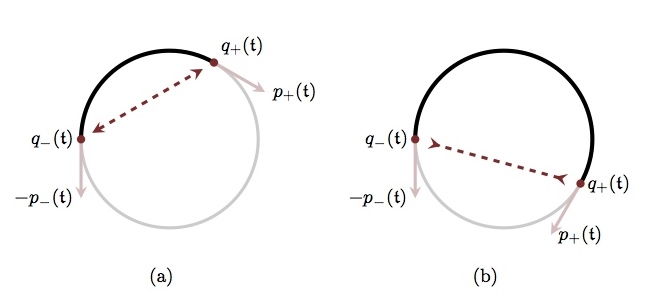
\includegraphics[scale=0.5]{cropped_nuts_image}

$x^Ty > 0 $ equivalent vectors form an acute angle.

\[p_{+}^T (q_+ -q_-) < 0 \Leftrightarrow p_+^T (q_- - q_+) > 0 \]

\[p_{-}^T (q_+ -q_-) < 0 \Leftrightarrow -p_-^T (q_+ - q_-) > 0 \]

Generalized No U-Turn sampler termination criterion:
\begin{align*}
 p_{+}^T (q_{+} -q_{-})  
 &=p_{+}^T \int_{t=0}^{T} M^{-1}p(t) dt   \\
 &=p_{+}^T M^{-1} \int_{t=0}^{T} p(t)dt \\
 &=(M^{-1} p_{+})^T  \int_{t=0}^{T} p(t)dt \\
 &= p^{\#}_{+}  \int_{t=0}^{T} p(t)dt \\
 &\approx p^{\#}_{+} \sum_{i=0}^n p(t_{k_i}) \\
 &=  p^{\#}_{+} \sum_{z \sim \mathbf{t}} p(z) \\
\end{align*}
 
\begin{algorithm}
  	\DontPrintSemicolon
	\SetKwFunction{FBuildTree}{G-BuildTree}

    \KwIn{initial position $q^0$, step size $\epsilon$, joint density $\pi$} 
    Re-sample $p^0 \sim \mathcal{N}(0,\mathbb{I})$ \;
    Initialize $q^{-} = q^0 , q^{+} = q^0 , p^{-} =p^0 , p^+ = p^0, p^+_{\#} = M^{-1}p^+,p^-_{\#} = M^{-1}p^-, p_s = p_0 j =0 ,	q^{next} = q^0 , s = 1 , w = \pi(q^0,p^0)$ \;
    \While{$s=1$}{
    Choose a direction $v_j \sim \text{Uniform}(-1,1) $ \;
    \eIf{$v_j = -1$}{
    		$q^-,p^-,-,-,q',s',w',p_{s'} \leftarrow \text{G-BuildTree}(q^-,p^-,v_j,j,\epsilon)$\;
    }{
    		$-,-,q^+,p^+,q',s',w',p_{s'} \leftarrow \text{G-BuildTree}(q^+,p^+,v_j,j,\epsilon)$\;
    }
    \If{$s'=\text{True}$}{
    		With probability $\min(1,\frac{w'}{w})$, set $\theta^{next} \leftarrow q^-$\;
    		$p_{s} = p_{s} + p_{s'} $\;
    		$p^\sharp_{+} \leftarrow M^{-1} p_{+} $\;
		$p^\sharp_{-} \leftarrow M^{-1} p_{-} $\;
    		
    		
    }
    $ w = w + w'$\;
    $ s = s' \mathbb{I}[(q^+ - q^-) \cdot p^\sharp_{-} \ge 0 ] \mathbb{I}[(q^+ - q^-) \cdot p^\sharp_{+}  \ge 0 ] $\;
    $j = j+1 $ \;
    
    }

\KwRet{$\theta^{next}$}

\FBuildTree{$\theta, r, v, j, \epsilon$}{\;
        \eIf{$j=0$}{
Base case: take one step in direction $v$ \;
$ q' , p' \leftarrow \text{Leapfrog}(q,p,v\epsilon) $ \;
$ w' \leftarrow \pi(q',p') $ \;
$s' = \text{True}$ \;
\KwRet{$q',p',q',p',q',s',w',p_{s'}$} \;

}{
	$p_s = 0 $\;
	$q^-,p^-,q^+,p^+,q',s',w',p_{s'} \leftarrow \text{G-BuildTree}(q,p,v,j-1,\epsilon) $ \;
	
	\If{$s'=\text{True}$}{
		$p_s = p_s + p_{s'}$\;
		\eIf{$v=-1$}{
			$q^-,p^-,-,-,q'',s'',w'',p_{s''} \leftarrow \text{G-BuildTree}(q^-,p^-,v,j-1,\epsilon)$ \;
		}{
			$-,-,q^+,p^+,q'',s'',w'',p_{s''} \leftarrow \text{G-BuildTree}(q^+,p^+,v,j-1,\epsilon)$ \;
		}
		\If{$s''=\text{True}$}{
		
		With probability $\min(1, \frac{w''}{w'+w''})$ , set $\theta' = \theta''$. \;
		$p^\sharp_{+} \leftarrow M^{-1} p_{+} $\;
		$p^\sharp_{-} \leftarrow M^{-1} p_{-} $\;
		$ s' \leftarrow s'' \mathbb{I}[(q^+ - q^- )\cdot p^\sharp_{-} \ge 0 ] \mathbb{I}[(q^+ - q^- )\cdot p^\sharp_{+} \ge 0 ]$ \;
		$w' \leftarrow w' + w'' $ \;
		$p_{s} = p_{s} + p_{s''} $\;
		
		}
	}
	\KwRet{$q^-,p^-,q^+,p^+,q',s',w',p_{s'}$}\;
}
    }
\caption{Generalized No U-Turn Sampler Update}
\end{algorithm}


Exhaustive Hamiltonian Monte Carlo termination criterion:

The Exhaustive Hamiltonian Monte Carlo termination criterion (XHMC) relies on significant amount of differential geometry for its justification. So the paper might read "an exhaustion ,$T_{\delta}(z)$, is the family of integration times in the contangent bundle such that the temporal change of the virial along the resulting Hamiltonian flow is uniformly bounded". Understanding fully the mathematics behind it is beyond the scope of this thesis. From my understanding it is a proxy to to monitor the return of a leapfrog trajectory to a neighbourhood around its initial point after having explored the energy level set. With a smaller threshold meant to push the neighbourhood smaller, hence forcing the exploration to continue for longer. Luckily the numerical quantities that needs to be computed are quite easily understood. In the original paper \cite{betancourt2016identifying}, the author showed improved sampling over the NUTS criterion as indicated by increased effective sample size on correlated distributions. 

The XHMC termination criterion is defined as follows: given a threshold $\delta > 0$, terminates simulation when 
\[  \Bigl |\frac{1}{|\mathbf{t}|} \sum_{z \in \mathbf{t}} \mathbb{P}[z | \mathbf{t}] \frac{dG}{dt}(z) \Bigr | < \delta \]

where 
\[ \mathbb{P}[z| \mathbf{t}] = \frac{\exp^{-H(z)}}{\sum_{z' \in \mathbf{t}} \exp^{-H(z')}} \]

The sum can be interpreted as a numerical approximation of an integration over the Hamiltonian flow $\phi_{t}^H(z)$

\[ \lim_{|\mathbf{t}| \rightarrow \infty} \frac{1}{|\mathbf{t}|} \sum_{z \in \mathbf{t}} \mathbb{P}[z | \mathbf{t}] \frac{dG}{dt}(z)  = \lim_{T \rightarrow \infty} \frac{1}{T} \int_0^T dt \frac{dG}{dt} \circ \phi_{t}^H(z) = 0 \]

\begin{align*}
 \frac{dG}{dt} &= \frac{d}{dt}\sum_{i=1}^D q_i p_i \\
 &= \sum_{i=1}^D p_i \frac{dq_i}{dt} + q_i \frac{dp_i}{dt} \\
 &= \sum_{i=1}^D [M^{-1}p]_i p_i - q_i \frac{\partial V}{\partial q_i} \\
 &= 2 T - q \cdot \frac{\partial V}{\partial q} \\
\end{align*}

\begin{algorithm}
  	\DontPrintSemicolon
	\SetKwFunction{FBuildTree}{XHMC-BuildTree}

    \KwIn{initial position $q^0$, step size $\epsilon$, joint density $\pi$} 
    Re-sample $p^0 \sim \mathcal{N}(0,\mathbb{I})$ \;
    Initialize $q^{-} = q^0 , q^{+} = q^0 , p^{-} =p^0 , p^+ = p^0, j =0 ,	q^{next} = q^0 , s = 1 , w = \pi(q^0,p^0), \text{ave} = \frac{dG}{dt}(q^0,p^0)$ \;
    \While{$s=1$}{
    Choose a direction $v_j \sim \text{Uniform}(-1,1) $ \;
    \eIf{$v_j = -1$}{
    		$q^-,p^-,-,-,q',s',w',\text{ave}' \leftarrow \text{XHMC-BuildTree}(q^-,p^-,v_j,j,\epsilon)$\;
    }{
    		$-,-,q^+,p^+,q',s',w',\text{ave}' \leftarrow \text{XHMC-BuildTree}(q^+,p^+,v_j,j,\epsilon)$\;
    }
    \If{$s'=1$}{
    		With probability $\min(1,\frac{w'}{w})$, set $\theta^{next} \leftarrow q^-$\;
    }
    $ Update \text{ave} by incorporating \text{ave}' $\;
    $ w = w + w'$\;
    $ s = s \mathbb{I}[ \frac{1}{2^j} |\text{ave} | < \delta ] $\;
    $j = j+1 $ \;
    
    }

\KwRet{$q^{next}$}

\FBuildTree{$q, r, v, j, \epsilon$}{\;
        \eIf{$j=0$}{
Base case: take one step in direction $v$ \;
$ q' , p' \leftarrow \text{Leapfrog}(q,p,v\epsilon) $ \;
$ w' \leftarrow \pi(q',p') $ \;
$ \text{ave}' \leftarrow \frac{dG}{dt}(q',p') $\;
\KwRet{$q^-,p^-,q^+,p^+,q',s',w',\text{ave}'$} \;

}{
	$q^-,p^-,q^+,p^+,q',s',w',\text{ave}' \leftarrow \text{XHMC-BuildTree}(q,p,v,j-1,\epsilon) $ \;
	
	\If{$s'=1$}{
		\eIf{$v=-1$}{
			$q^-,p^-,-,-,q'',s'',w'',\text{ave}'' \leftarrow \text{XHMC-BuildTree}(q^-,p^-,v,j-1,\epsilon)$ \;
		}{
			$-,-,q^+,p^+,q'',s'',w'',\text{ave}'' \leftarrow \text{XHMC-BuildTree}(q^+,p^+,v,j-1,\epsilon)$ \;
		}
		With probability $\min(1, \frac{w''}{w'+w''})$ , set $q' = q''$. \;
		Update $ave$ by incorporating $w'$ and ${ave}'$ \;
		$ s' \leftarrow s'' \mathbb{I}[(q^+ - q^- )\cdot p^- \ge 0 ] \mathbb{I}[(q^+ - q^- )\cdot p^+ \ge 0 ]$ \;
		$w' \leftarrow w' + w'' $ \;
	}
	\KwRet{$q^-,p^-,q^+,p^+,q',s',w',{ave}'$ }\;
}
    }
\caption{Exhaustive Hamiltonian Monte Carlo Sampler Update}
\end{algorithm}


xhmc over gnuts over nuts 
\section{Adaptive Tuning of Step Size}

Setting the stepsize that makes the leapfrog mapping stable.

Analysis: For one dimensional potential energy function $V(q) = \frac{q^2}{2\sigma^2}$,
that is, normal distributed with variance $\sigma^2$. Writing out the matrix that encodes the linear mapping from $(q(t),p(t))$ to $(q(t+\epsilon),p(t+\epsilon))$ gives that the mapping is stable if $\epsilon < 2 \sigma$, and diverges otherwise. 

For the general multivariate $q$ with arbitrary potential energy function, equivalent to a general density fucntion, we approximate the potential energy function with a second order taylor expansion, so that the $q^2$ term in the taylor expansion of $V(q)$ has coefficient $\frac{1}{2} \frac{\partial^2 V}{\partial q^2}$  
By matching the two expressions we get 
\[ \sigma \approx ( \frac{\partial^2 V}{\partial q^2})^{-1/2} \]

So by setting $\epsilon$ to that value, we are exactly in the middle of the domain of allowable stepsizes, equivalent to half of the boundary limit.
Care has to be taken to note evalue the second derivative using values of the current parameters, because then the leapfrog steps are no longer reversible (i.e. get different stepsizes at two ends of a trajectory. So when you reverse direction at the other end you don't return to  the starting point). 

This is only useful if you are doing a sort of blocks gibbs sampling, where you use HMC to sample from the low-level paramters while keeping the hyperparameters fixed, then sample the hyperparameters while keep the parameters fixed. 

Might be much more difficult to select stepsize if we don't do this. Try to use Riemmanian Monte Carlo to overcome skewness of joint distribution of hyperparameters and parameters. 

same as nuts paper 



Now we describe how the stepsizes are automatically tuned in STAN. First, keep
in mind that the stepsize is adapted only during the warmup phase and stays
fixed during the sampling phase. This ensures the correctness of the algorithm
as the induced Markov chain resulted from an adaptive stepsize may not be
reversible. One way of manual tuning is try to find the stepsize
$\epsilon'$ that would result in an acceptance probability of $0.65$. The
acceptance probabiilty is an averaged quantity, calculated as an expectation
over a chain. That is, we try to optimize $\epsilon \in \mathbb{R}$ with respect
to the function 
\[ h(\epsilon) = E_\pi[f(X)|\epsilon]  = \lim_{T \rightarrow \infty} \frac{1}{T}
\sum_{t=1}^T E[f(X_t)|\epsilon] \]

where $f(X_t)$ denotes the acceptance probability for iteration $t$. The
second equality comes from the convergence of the MCMC sampler. This is a
stochastic optimization problem, and STAN uses the dual averaging scheme of
Nesterov compute the stepsize. The dual averaging scheme works in general as
follows, supose we are trying to find $x\in \mathbb{R}$ such that $h(x) =
E[H_t|x] = 0$ then we perform the updates 

\[x_{t+1}  = \mu - \frac{\sqrt{t}}{\gamma} \frac{1}{t+t_0} \sum_{i=1}^tH_i;
\bar{x}_{t+1} = \eta_t x_{t+1} + (1-\eta_t) \bar{x}_t \]

where $\mu$ is the target that the $x_t$'s are shrunk towards, $\gamma > 0$ a
paramater that controls the amount of shrinkage, $t_0 \ge 0$ a parameter that
stablizes the early iterations, and $\eta_t = t^{-\kappa},\kappa>0$ is a
stepsize schedule ensuring convergence. Since $\epsilon>0$, this is technically
a constrained optimization problem, but it can be easily converted into an
unconstrained problem by optimizing for $\log(\epsilon)$ instead. 

\begin{algorithm}
\KwIn{Target Metropolis acceptance rate $\delta$, initial step size $\epsilon_0$, duration of tuning $M^{adapt}$ }

Initialize $\overline{H}_0 = 0, \gamma = 0.05, t_0 = 10 ,\kappa = 0.8 $ \;
	
	Calculate acceptance rate $\alpha$ using $\epsilon_0$. \;
\For{$m = 1:M^{adapt}$}{
	 $\overline{H}_m = (1- \frac{1}{m+t_0}) \overline{H}_{m-1} + \frac{1}{m + t_0} (\delta - \alpha) $ \;
	 $\log \epsilon_m = \mu - \frac{\sqrt{m}}{\gamma} \overline{H}_m $ \;
	 $\log \overline{\epsilon}_m = m^{-\kappa} \log \epsilon_m + (1-m^{-\kappa}) \log \overline{\epsilon}_{m-1} $ \;
	
	Update acceptance rate $\alpha$ using $\overline{\epsilon}_m$ \;
	
}

\caption{dual averaging tuning of $\epsilon$ }
\end{algorithm}


\begin{algorithm}
Initialize $\epsilon = 1$, momentum $p \sim \mathcal{N}(0,\mathbb{I}) $ \;
$(q',p') \leftarrow \text{Leapfrog}(q,p,\epsilon) $ \;
$a \leftarrow 2 \mathbb{I}[ \frac{\pi(q',p')}{\pi(q,p)} > 0.5 ] -1 $\;
\While{ ( $\frac{\pi(q',p')}{\pi(q,p)} )^a > 2^{-a} $}{
	$\epsilon \leftarrow 2^a \epsilon$ \;
	$(q',p') \leftarrow \text{Leapfrog}(q,p,\epsilon) $ \;
}
\KwRet{$\epsilon$}
\caption{find initial $\epsilon$} 
\end{algorithm}

\section{Adaptive Tuning of HMC Metric}
STAN divides the tuning period into a number of windows of different lengths. The following quantities followed by their current default values in brackets are of relevance in this discussion: 

\begin{enumerate}
\item Initial buffer (n=75): the first window of the sampling stage, where only the step size parameter is updated by dual averaging .

\item End buffer (n=50): the last window of the sampling stage, where the covariance metric is fixed and only the step size is updated and allows it to stabilize.

\item Window size (n=25): the base length of interval for updating the covariance metric. 
\end{enumerate}

Both the step size and covariance metric are updated during the tuning stage. And it proceeds as follows: the covariance metric is initialized by the identity matrix and an initial step size found by the doubling-halving heuristic. Parameter tuning happens in three stages. The first is the initial buffer where only $\epsilon $ is updated. In the second stage both the step size and covariance metric are updated. While $\epsilon$ is updated after every MCMC transition, because the dual averaging procedure only requires an acceptance rate, the covariance metric is updated only after the number of MCMC samples collected is equal to the current window size. Then compute the empirical covariance and set the metric to its inverse. Double the window size or increase it to cover the rest of the remaining second stage if doubling is impossible. The third and last stage updates the step size only. 

The algorithm is designed so that the covariance metric is not updated immediately at the start of the tuning stage, because the model might be initialized particularly poorly and hence the initial examples could be misleading. The doubling of window size is to allow progressive improvement of the covariance metric. For larger window sizes, the memory requirement for storing all the MCMC samples to estimate the covariance matrix could be prohibitive. Therefore, STAN actually uses an online algorithm for calculating the covariance, whose memory complexity is independent of the window size. 

\section{HMC-Specific Sampling Diagnostics}
bfmi , divergence ( talk about example 8 school) , tree depth ,

First we describe how it uses
divergence to diagnose $\epsilon$'s that are too large. First, a large constant
is selected $Th = 1000$, then after each proposal $(x_i,y_i)$, we compare the
energy value $H(x_i,y_i)$ with that of the previous state $H(x_{i-1},y_{i-1})$,
if $|H(x_i,y_i) - H(x_{i-1},y_{i-1})|> Th$ then a divergence is flagged and the
proposal rejected. At the end of the sampling stage, the total number of
divergence indicates potential problem with the chosen stepsize. Typically the
only resposne available is to reduce the stepsize and slow down sampling,
although persistent divergence may call for reparametrization as the parameter
space may have many sharp edges and steep wells that no stepsizes are small
enough to navigate the space. The existence of divergence implies the samples
drawn may be biased and hence invalid. This is not a diagnostic to be ignored.

The second diagnostic tool that comes with STAN is the Bayesian fraction of
missing information (BFMI). It detects a mismatched conditional Hamiltonian
energy function
distribution to the marginal Hamiltonian distribution. The leapfrog step is
restricted to exploring a level set determined by the 
initial positions $(q_i,p_i)$ at the start of the trajectory. Given the previous
state $q_i$, the only randomness comes from the resampling of the auxillary
momentum distribution. Since the goal is
to explore the entire parameter space, we want the two energy distributions to
closely match each other. BFMI allows us to measure that match. Formally it is defined as 
\[ BFMI = \frac{ E_\pi[Var_{\pi_{H|q}}[H|q]]}{Var_{pi_H}[H]} \]
where $\pi$ is the marginal distribution of $q$ and $\pi_{E|q}$ and $\pi_{H}$
are the conditional and marginal distributions of the Hamiltonian energy
function $H$ respectively. In practice the expectations must be estimated, but
it is easily done by evaluting the energy function at the values coming from the
generated Markov chain. Suppose $N+1$ samples are drawn, 

\[ \hat{BFMI} = \frac{\sum_{n=1}^N(H_n-H_{n-1})^2}{\sum_{n=0}(H_n-\bar{H})^2} \]
where $H_n = H(q_n,p_n)$ and $\overline{H}=\frac{1}{N+1}\sum_{n=0}^N H_n$. From basic
probability we have $0 \le BFMI \le 1 $ and the optimal value is when it is
1. A low value of $\hat{BFMI}$ suggests that the auxillary momentum distribution is
inefficient for sampling. 

 
\section{Other Sampling Diagnostics}
ess gelman definition, rhat 
Potential scale reduction : factor by which the scale of the current distribution for $\psi$ might be reduced if the simulations were continued in the limit $n \rightarrow \infty$. This quantity should converge to $1$ as $n \rightarrow \infty$. If $\hat{R}$ is high, $ > 1.1 $, for example, we might we want to continue simulation. 

\begin{align*}
&B = \frac{n}{m-1} \sum_{j=1}^{m}(\overline{\psi}_{\cdot j} - \overline{\psi}_{\cdot \cdot})^2, \text{ where } 
\overline{\psi}_{\cdot j} = \frac{1}{n} \sum_{i=1}^n \psi_{ij} , \overline{\psi}_{\cdot \cdot} = \frac{1}{m} \sum_{j=1}^m \overline{\psi}_{\cdot j }
 \\
&W = \frac{1}{m} \sum_{j=1}^m s_j^2 , \text{ where }
s_j^2 = \frac{1}{n-1} \sum_{i=1}^n (\psi_{ij} - \overline{\psi}_{\cdot j } )^2.\\
\end{align*}

\[ \hat{\text{var}}^+(\psi|y) = \frac{n-1}{n} W + \frac{1}{n} B \]

\[\hat{R} = \sqrt{\frac{\hat{\text{var}}^+(\psi|y)}{W}} \]

ESS 
\[n_{eff}  = \frac{mn}{1 + 2 \sum_{t=1}^\infty \rho_t} \]

\[V_t = \frac{1}{m(n-t)} \sum_{j=1}^m \sum_{i=t+1}^n (\psi_{i,j} - \psi_{i-t,j})^2 \]

$E[(\psi_i - \psi_{i-1})^2] = 2(1-\rho_t)\text{var}(\psi)$

\[\hat{\rho}_t = 1 - \frac{V_t}{2 \hat{\text{var}}^+}\]


\[\hat{n}_{eff} = \frac{mn}{1 + 2 \sum_{t=1}^T \hat{\rho}_t} \]
 


\section{Numeric tricks/Implementation tricks}

$\pi(q,p)  = \exp(H(q,p)) $

$\frac{\pi(q',p')}{\pi(q,p)} )^a > 2^{-a} $

Equivalent to 

$ a (H(q',p') - H(q,p) ) > -a \log 2 $ 

cov add unity 0.0001 + welford

Covariance added dimension unity matrix.

\begin{algorithm}
\DontPrintSemicolon
\KwIn{current sample counter $t$, current accumulator for mean $m$, current accumulator for $m_2$, current sample $x$}

$\delta = x-m$ \;
$m = m + \frac{\delta}{t} $\;
$m_2 = (x-m)\delta^T $ \;
$\mu = m $\;
$\Sigma = \frac{m_2}{t-1} $\;
\KwRet{$m,m_2,\mu,\Sigma$}
\caption{Welford algorithm}
\end{algorithm}

logsumexp
\begin{algorithm}
\DontPrintSemicolon
\KwIn{$a,b$}
\KwOut{$c = \log(\exp(a)+ \exp(b)) $}
$s = \max(a,b) $\;
$c = s + \log( \exp(a-s) + \exp(b-s)) $\;

\KwRet{$c$}
\caption{logsumexp}
\end{algorithm}


stable sum 
\begin{algorithm}
\DontPrintSemicolon
\KwIn{$a_1,\log w_1 , a_2, \log w_2$}
\KwOut{$a = \frac{a_1 \log w_1 + a_2 \log w_2}{w_1+w_2} ,w = w_1 + w_2$}

\eIf{$\log w_1 > \log w_2 $}{
	$e = \exp(\log w_1 - \log w_2 ) $\;
	$a = \frac{e \cdot a_1 + a_2}{1+e} $\;
	$w = \log w_2 + \log(1+e) $ \;
}{
	$e = \exp(\log w_2 - \log w_1 ) $\;
	$a = \frac{e \cdot a_2 + a_1}{1+e} $\;
	$w = \log w_1 + \log(1+e) $ \;
}


\KwRet{$a,w$}
\caption{Stable Sum }
\end{algorithm}

divergence check 
recursion requiring dynamic graph  > pytorch
version of nuts that takes care of divergence
fft variogram

map from unconstrained space to constrained space

Suppose $ X = exp(y) $  
\begin{align*}
p_Y(y) = p_X(f^{-1}(y)) \ |\frac{d}{dY} f^{-1}(y) |\\
p_Y(y) = p_X(\exp(y)) \cdot \exp(y) \\
\log p_Y(y) = \log p_X(\exp(y)) + y \\
\end{align*}

\begin{align*}
 \sum_{n=t+1}^N (\theta_{n} - \theta_{n-t})^2 &= \sum_{n=t+1}^N \theta_n^2 - 2 \theta_n \theta_{n-t} + \theta_{n-t}^2  \\
 &= \sum_{n=t+1}^N \theta_n^2 -2 \sum_{n=t+1}^N \theta_n \theta_{n-t} + \sum_{n=t+1}^N \theta_{n-t}^2 \\ 
  &= \sum_{n=t+1}^N 1 \cdot \theta_n^2 -2 \sum_{n=t+1}^N \theta_n \theta_{n-t} + \sum_{n=t+1}^N 1 \cdot \theta_{n-t}^2 \\
\end{align*}


Debug MCMC sampler. Match mean and covariance. Question: how close is close enough?

Suppose we want to sample from a bivariate normal distribution with known mean and covariance matrix. Say $\mathcal{N}(\mu,\Sigma) $, where 

\begin{displaymath}
\mathlarger{\Sigma} = 
\begin{bmatrix}
\sigma^2_1 &\sigma_{12}^2 \\
\sigma_{21}^2 &\sigma^2_2 \\
\end{bmatrix}
\end{displaymath}

Given a chain of $n$ MCMC samples $\{x_i\}_{i=1:n}$ generated by the sampler to be tested, we could estimate  the target mean by $ \frac{1}{n-1} \sum_{i=1}^ n x_i$. Since $E[X-\mu] = 0$, we would expect the generated quantity $\eta= \frac{1}{n-1} \sum_{i=1}^ n x_i -\mu$ to decrease with increasing number of samples. We could monitor $\eta$ by comparing it with its Monte Carlo standard error (MCSE) 

\[ \text{MCSE} = \frac{\hat{\sigma}}{\sqrt{n_{\text{eff}}}} \]

where $\hat{\sigma}$ is the estimated standard deviation. By the Central Limit Theorem one would expect  $\eta \in (-\text{MCSE},\text{MCSE})$ with high probability. 

Similarly we can monitor quantities like $\frac{1}{n-1} \sum_{i=1}^n ({x_i}_1 -\mu_1)^2 - \sigma^2_1,  \frac{1}{n-1}^n \sum_{i=1}^n ({x_i}_1 - \mu_1)({x_i}_2 - \mu_2)^2 $ to assess convergence to the marginal variances and covariance.

One can then construct example models where the mean and covariance are known explicitly, simulate multiple chains and monitor quantities for approximate convergence, in the sense that the empirical estimated quantities differ from their exact quantities by a margin no larger than its MCSE (or its constant multiple .) 

\chapter{Bayesian Neural Networks}
\section{Neal}

Deep learning, a field in machine learning studying multilayered neural network models, has become quite successful in artificial intelligence tasks and a lot of research has been, and is currently underwayto improve our understanding of these models and apply them better and to more fields. See \cite{Goodfellow-et-al-2016-Book,lecun2015deep} a general introduction into the methodology and application of deep learning, and \cite{schmidhuber2015deep} for an in-depth literature review. It is futile to attempt a complete overview of the field because it is too vast but we will provide some pointers that reflect what the author finds important and some motivations. 

Before there was deep learning, a term which only came about in the mid 2000s, there were Neural Networks \cite{bishop1995neural,ripley2007pattern}, which were also hugely popular in the 90s, but ultimately could not scale up. The main reason for this was the difficulty of training neural networks of more than one or two hidden layers. Traditional optimization techniques like stochastic gradient descent with backpropogation did not improve empirical test error for networks with more layers,not until ideas like pre-training to initialize optimization were experimented could we fit "deep" neural networks with more than 2 hidden layers. This restarted the field, now rebranded as Deep learning, and innovations like using the rectified linear units as activation functions \cite{nair2010rectified} to allow training deep networks without pre-training, and using GPUs to speed up practical training process \cite{krizhevsky2012imagenet}, as well as the creation of numerical libraries like Theano \cite{bergstra2010theano}, Caffe \cite{jia2014caffe}, Tensorflow\cite{tensorflow2015-whitepaper}, to name a few, that make building and training neural network models much easier by automating the backpropogation step with symbolic differentiation \cite{bahrampour2015comparative} and handles the transition between CPU and GPU computation modes. 

Suppose we have $n$ observed datapoints $\{y_i,x_i\}$ where $X_i \in
\mathcal{R}^p$ is a $p$-dimensional vector, then a neural network models the
data as follows:

\[y_i = \prod_{j=1}^Lg_j(V_jf_j(W_j))x_i \]
where $L$ is the number of layers of the network, $W_j$ a $n_j \times m_{j-1}$
weight matrix, $V_j$ a $m_j \times m_{j-1}$ weight matrix, and each $g_j$,$f_j$
a pair of activation functions that are usually non-linear functions. There are
usually no restrictions on what these activation functions must be other than on
$g_L$ which must match the data type of the $y_i$'s. For example, if $y_i$ are
binary observations then we would like the last output activate function to be a
logistic function so that it maps output to strictly $[0,1]$, just like in
logistic regression.

Popular activation functions in the classical neural network literature includes
the logistic function and the hyperbolic tangent function, but in modern deep
learning the Rectified linear unit (RELU) has come to dominate the field. It has
a simple form of $g(x)=\max{0,x}$, which is straightforward to do
backpropogation with despite a single point of nondifferentiability, and it was
found to improve optimization enormously. It's discovery has allowed training
neural network models with many more layers than 2 with random initialization of
weights, getting rid of the need for pre-training. 

While neural networks can have different number of layers and number of hidden
units within each layer, theoretically only one layer is sufficient to
approximate any function as we increase the number of hidden units \cite{hornik1991approximation}. 

For Bayesian neural networks, where one put a Gaussian prior distribution on the weights of model, it has been shown that for a one-hidden-layer model, the prior converges to a Gaussian process as the number of hidden units converge to infinity \cite{neal2012bayesian}.This gives a neat intrepretation of bayesian neural networks. 

Further work by \cite{gal2015dropout}, shows that heuristic training techniques such as dropout are actually are actually doing variational inference with Deep Gaussian Process \cite{damianou2013deep}, a process where several GPs are stacked one after another. 

The most exact way to perform bayesian inference for BNNs is still MCMC sampling as pioneered in Neal's thesis. In his work he put a hiearchical prior on the weights of the network and sampled the weights with HMC and the hyperparameter with block-Gibbs updates. One of his graduate students attempted tosample both of the weights and hyperparameters with HMC but did not get better performance, mostly because of the highly skewed distribution common in hierarchical models. With the invention of RMHMC and its successful application to sample more efficiently from hierarchical models, it would be interesting to try to see if this method can be adapted to sample from the posterior distribution of a BNN. 

For some theory on why, for the same number of hidden layers, it would be better to have multiple layers in a NN rather than a wide single-layer network, see \cite{montufar2014number}. 

typical model 
i.e. windowed hmc, hand tuning, ard priors.  Refer back to NUTS for discussion  of windowed hmc . 
multimodality convergence concern P v NP

\section{gibbs vs joint sampling}
Suppose $W_{ij} \sim \mathcal{N}(0,\sigma^2), \sigma^{-2} \sim \text{Gamma}(a_0,b_0) $

Then , $n = |W|$ 
\[\sigma^{-2}|W,X,y \sim \text{Gamma}(a_1,b_1)\]
\[a_1 = a_0 + 0.5 n  \]
\[b_1 = b_0 + 0.5 \sum_{ij} W_{ij}^2 \]

\begin{algorithm}
\KwIn{Initial variance $\sigma^2_0$, number of MCMC samples $M$}

\For{$ i = 1:M$ }{
	Sample $W_i \sim p(W|\sigma^2_{i-1},data)$ \;
	$a_1 = a_0 + 0.5 n $ \; 
	$b_1 = b_0 + 0.5 \sum_{ij} W_{ij}^2$ \;
	Update $\sigma^2 \sim \text{Inv-Gamma}(a_1,b_1)$ \;
}
\KwRet{$W_{i=1:M}$}
\caption{Blocks-Gibbs Sampler for NN weights and variance}
\end{algorithm}



describes gibbs as done by neal 
i.e. tried joint sampling, ncp 
side tracked to talk about cp vs ncp 
\section{SGHMC}
tried on mnist
The idea of simulating Hamilotnian dynamics without the metropolis acceptance step was first experimented in the statistics/machine learning literature by Neal \cite{neal1993bayesian} in a batch MCMC sampler for the posterior distribution of a BNN. He found that with careful selection of the leapfrog stepsize, the biased samples achieve similar predictive performance as the full MCMC samples. Therefore, it seems to suggest that for predictive tasks .e.g. regression or classificaiton where observations are abundant, we could 
use a validation set (predictive performance) to select tuning parameters, hoping to achieve trade off a bit of bias for better predictive performance. 
Tie in with stochastic gradient descent hamiltonian monte carlo
Another trick that helps to speed up the HMC sampler is data subsampling, also denoted partial gradient in Neal's thesis \cite{neal2012bayesian}.
Assuming there are $n$ data points, the potential energy function $V(q)$ can be written as 
\[ V(q) = -\log( \pi(q) \pi(q|data) = -\log(\pi(q)) -\log \pi(q|data) = -\log(\pi(q)) - \sum_{i=1}^n \log \pi(q|data_i) \]
where $\pi(q)$ is the prior density function and $\pi(q|data)$ is the likelihood function. Note that the finite series in the last expression above can be approximated as 
\[ \sum_{i=1}^n \log \pi(q|data_i) \approx \frac{n}{k} \sum_{i \in I} \log \pi(q|data_i) \]
where $I$ is a subset of $\{1,\dots, n\}$ of size $\frac{k}{n}$. 
More pratically, if we divide the datapoints into $M$ equally sized subsets. Then for any such subset $S$, the potential energy function can be approximated by 
\[ V(q) \approx    -\log(\pi(q)) + M \sum_{i \in S} \log(\pi(q|data_i)) \]


In modern deep learning, fitting of neural network models usually is done by stochastic gradient descent (SGD) \cite{ngiam2011optimization}.
This is exactly the same as regular gradient descent \cite{wright1999numerical}, except at each weight update and random subset(batch) of datapoints are sampled to be the full observations, and the sequence of stepsizes over the optimiztion process must decrease while satisfying the property

\[ \sum_{t=1}^\infty \epsilon_t = \infty , \sum_{t=1}^\infty \epsilon_t^2 < \infty \]

Theory from the stochastic optimization literature \cite{robbins1951stochastic} guarantees convergence to a local minimum. However, as per the norm in the optimization literature, the convergence property is usually only provable for easier classes of problems (.e.g. convex, quadratic functions) to which the likelihood of neural network models does not belong. Nonetheless, SGD has the advantage of easy implementation and low memory requirement (O(p)), and hence remains the dominant optimization method in deep learning.  

The success of SGD lies in being able to avoid evaluating the full likelihood, which has contribution from each data point, at each update. The problems that neural network models tend to be fitted are usually in the high-sample-size, high-dimensional regime, hence a full evaluation would slow down the algorithm significantly. A stochastic gradient extension to MCMC was first experimented by \cite{welling2011bayesian}, where the author proposed to use the following updates :

\[q_{t+1} = q_t + \frac{\epsilon_t}{2} ( \nabla \log p(q_t) + \frac{N}{n} \sum_{i \in D} \nabla \log \pi(x_i|q_t) ) + \eta_t , \eta \sim \mathcal{N}(0,\epsilon_t) \]

where $D$ is a random subset of $\{1,2, \dots, N\}$ of size $n$ sampled at each update of $q$. We assume there are $N$ observations in total. The stepsizes are assumed to decay following the constraint stated above for SGD. The authors recommended setting $\epsilon_t = a(b+t)^{-\gamma} $ with $\gamma \in (0.5,1]$.  

Marginal predictive distributions or any expectation taken with respect to the posterior distribution can be calculated by 
\[ E[f(q)] \approx \sum_{t=1}^M \epsilon_t f(q_t) / \sum_{t=1}^M \epsilon_t \] 
This estimator has lower variance than the naive alternative $\frac{1}{M} \sum_{t=1}^M f(q_t) $ and is unbiased as well. 

The author proved that as the stepsizes $\epsilon_t$ goes to $0$ the samples $\{q_t\}$ converge tothe Langevin dynamics targeting the posterior distribution. Of course, in practice we set lower bound on $\epsilon_t$ and stop decreasing the stepsize once it is small enough. Also, the fact the we are not doing the acceptance-rejection step means there will be a bias in our posterior samples, which unlike the samples drawn from a Metropolis-Hastings sampler, does not decrese to $0$ as we sample from the chain longer.



Simulating from the discrete approximation to a Langevin dynamics is the basis
for Langevin Monte Carlo or Metropolis adjusted Langevin Algorithm, which
includes an acceptance-rejection step at each update. This can also be seen as a
special case of HMC where only one leapfrog step is used ($L=1$). It has been
demonstrated that HMC is much more efficient than LMC because it avoids random
walk. (Show $O(D^{4/3})$ vs $O(D^{5/4})$ kind of results). This inspires
Stochastic Gradient Hamilotian Monte Carlo (SGHMC) ,
which extends HMC the way SGLD extends LMC. 

\begin{algorithm}
    \caption{Stochastic Gradient HMC}
    \KwData{Input: $\eta,\alpha,n,M,L,q_0$}
        Initialize $\theta_0,v_0$ \;
        \For{$t = 1:M$}{
        $q^{0}=q_{t-1}$\;
        $v^{0}=v_{t-1}$ \;
        
        \For{$i = 1:L$}{
        $q^{i} = q^{i-1} + v^{i-1}$ \;
        Sample $z \sim \mathcal{N}(0,2(\alpha-\hat{\beta} \eta)$ \;
        Sample minibatch and calculate $\nabla \tilde{V}(q)$  \;
        $v^{i} = -\eta \nabla \tilde{V}(q) - \alpha v^{i-1} + z$ \;
        }
        
        $q_t = q^{L}$ \;
        $v_t = v^{L}$ \;
        }
\end{algorithm}

Applying MCMC methods to large datasets often involve 2 problems. First, evaluating the unnormalized posterior density
\[ \pi(D|q) = \prod_{i=1}^n \pi(x_i|q) \]
 is equivalent to passing through all datapoints, which alone can make the sampling algorithm unacceptably slow since all versions of the Metropolis-Hastings sampler requires such evaluations for proposing new samples. Second, models that require MCMC samples when a large number of datapoints are available are necessarily singular models. Using the terminology of \cite{watanabe2009algebraic}, regular models are models for which the bayesian central limit theorem \cite{le2012asymptotic} holds, that is, when the number of observations goes to infinity the posterior distribution of $q$ converges to a Gaussian distribution. Models that are non-regular are called singular models. A lot of methods designed to scale MCMC \cite{neiswanger2013asymptotically,scott2016bayes,} ultimately rely on this asymptotic normality for validity. Bayesian logistic regression is a classical model for which the CLT holds and is used in many papers to demonstrate the effectiveness of newly proposed large-scale MCMC methods. However, the very fact that asympotitic normality holds means there is little added utility to drawing MCMC samples from the posterior distribution, since a normal approximation would suffice. On the other hand, for singular models there is no guarantee that the estimates converge to the target posterior distribution. 

Asympotic normality is also assumed for the application of stochastic gradient mcmc methods to neural network models \cite{welling2011bayesian,chen2014stochastic,ahn2012bayesian,ding2014bayesian,ma2015complete}. Even though neural networks are singular models where the conditions for the central limit theorem do not hold, these methods have shown good predictive performance on a variety of datasets. This is opposite of what one would expect and merits further investigation.







Now we review some important samplers in the stochastic gradient MCMC
literature. Stochastic Gradient Langevin Dynamics (SGLD) was first introduced by
\cite{welling2011bayesian}. 
Stochastic gradient Hamiltonian Monte Carlo
Got rid of the metropolis acceptance step. No longer sampling from the exact
distribution. Second order method, needs to estimate fisher information matrix.

\cite{chen2014stochastic}

Problem is you are not saving that much computation time if you now end up with a second-order method, and if you want to sample exactly from the target distribution you still have to evaluate the Hastings ratio using the entire dataset.

There is a tendency in the stochastic gradient MCMC literature to omit the Metropolis correction step.

See \cite{ding2014bayesian} 
Quote: "If the stationary distribution is not the target distribution, a Metropolis-Hastings (MH) correction can often be applied. Unfortunately, such correction steps require a costly computation on the entire
2
dataset. Even if one can compute the MH correction, if the dynamics do not nearly lead to the correct stationary distribution, then the rejection rate can be high even for short simulation periods h. Furthermore, for many stochastic gradient MCMC samplers, computing the probability of the reverse path is infeasible, obviating the use of MH. As such, a focus in the literature is on defining dynamics with the right target distribution, especially in large-data scenarios where MH corrections are computationally burdensome or infeasible.
"
\cite{ma2015complete}
This is total crazy talk (not sampling from the target distribution exactly!)

Perhaps if we can quantify the bias somehow we can make it work.

Note the data subsampling approach does not work for Gaussian Process models because of the calculation of the covariance inducing dependence among observations \cite{filippone2015enabling}.
\cite{teh2014consistency}
Proves consistency of SGLD despite throwing away Hastings ratio step. Tradeoff is slower exploration.

Stochastic gradient Hamiltonian Monte Carlo \cite{chen2014stochastic}
relies on the assumption that the gradient of the log target density is normally distributed, which in turn comes from assuming independence of the observations $x$ and appealing to the central limit theorem.

Same CLT assumption about the gradient is made in
the SGLD paper \cite{welling2011bayesian}.

Some more theory behind SGLD and SGHMC \cite{ma2015complete}
Stochastic gradient thermostat : an improvement on SGHMC by getting rid of the need to estimate a covariance matrix. 

First introduced here\cite{ding2014bayesian}, exteneded\cite{gan2015scalable} to have multiple thermostat parameters instead of just 1 in the original version, some analysis as well as introduction of a higher-order numerical integrator here\cite{li2015high,chen2015convergence}.

Preconditioned SGLD \cite{li2015preconditioned} uses information of the curvature. Can be thought of as extension of SGLD same way RHMC extends HMC. Does not use full Fisher information matrix. Uses diagonal approximation to reduce complexity.
Stochastic expectation propogation.

Stochastic gradient fisher scoring \cite{ahn2012bayesian}

Using stochastic gradient is only one way of scaling and automating MCMC. Also can try adaptive MCMC methods\cite{roberts2009examples}. Relevant dynamical versions include \cite{wang2013adaptive},where Bayesian optimization \cite{mahendran2012adaptive,snoek2012practicalx,} is used to tune the HMC sampler.

stochastic gradient quasi netwon langevin dynamics requires extra tuning paramters with little guidance on how to tune them \cite{csimcsekli2016stochastic}

preconditioned sgld introduces bias\cite{li2015preconditioned}.


Important points to retain: connection to sgd with momentum. dont know how to
set $C$ matrix. noise of gradient $B$ not actually estimated in any of the
examples in the paper claiming as stepsizes goes to zero the noise goes to zero
as well. The estimation can be done using along diagonal approximation, or  
low-rank approximations. 

\section{sparsity inducing priors}
horseshoe priors for model selection.

Horseshoe prior \cite{piironen2017sparsity}

\[ \mathbf{\beta} = (\beta_1,\cdots,\beta_D)\]

\begin{align*}
 &\beta_j \sim \mathcal{N}(0,\tau^2\lambda^2) \\
 &\lambda_j \sim C^+(0,1),\, j = 1,\dots , D, \\
\end{align*}

Talk about parametrization ncp 

Regularized horseshoe prior 

\begin{align*}
&\beta_j | \lambda_j, \tau, c \sim \mathcal{N}(0,\tau^2 \tilde{\lambda}_j^2) ,\, \tilde{\lambda}_j^2 = \frac{c^2 \lambda_j^2}{c^2 + \tau^2 \lambda_j^2} \\
&\lambda_j \sim C^+(0,1),\, j = 1,\dots,D\\
&c^2 \sim \text{Inv-gamma}(2,8) ,
\end{align*}

Relation to student-t distribution. 

Cauchy distribution equivalent to student-t distribution of degree 1. Also, if $x \sim t_{\nu}(0,1) $ 
equivalent to 
\[ x \sim \mathcal{N}(0,\sigma^2)\]
\[\sigma^2 \sim \text{Inv-gamma}(0.5,0.5) \]

Equivalent to 
\[ x = z * \sigma \]
\[ z \sim \mathcal{N}^+(0,1)\]
\[\sigma^2 \text{Inv-gamma}(0.5,0.5) \]

The parameter space becomes 

\[(z,r1_l,r2_l,r1_g,r2_g) \]
Where
\[ z \sim \mathcal{N}(0,1) \]
\[ {r_1}_l^j \sim \mathcal{N}^+(0,1) \, \forall j \]
\[ {r_2}_l^j \sim \text{Inv-gamma}(0.5,0.5) \, \forall j  \]
\[ {r_1}_g \sim \mathcal{N}^+(0,1)  \]
\[ {r_2}_g \sim \text{Inv-gamma}(0.5,0.5)   \]

\[ \lambda =  {r1}_l \cdot {r2}_l \]
\[ \tau = r1_g \cdot r2_g \]
\[\beta = z \cdot \lambda \tau \]

The unconstrained parameter space becomes $(z,\log r1_l,r2_l,\log r1_g,r2_g)$

\section{self normalizing induced initialization}
selu, gloriot initialization

\[ W \sim \text{Uniform}(\frac{-1}{\sqrt{N_{in}}},\frac{1}{\sqrt{N_{in}}}) \]

\section{model selection}
test error vs waic 
In a neural network model there are multiple hyperparameters left to be tuned be
the user. These include the number of hidden layers, the number of hidden
variables in each layer, the choice of activation functions, the use of
convolutional layers in the case of convolutional neural networks, the prior
distribution on the weights of the network. Each different combination of these
hyperparameters constitute a model choice. In the neural network literature,
usually a train-test dataset split is used. The full dataset with observations
$\{\textbf{y},\textbf{x}\}$ is split randomly into a training set
$\{\textbf{y}_{train}, \textbf{x}_{train}\}$ and a test set $\{\textbf{y}_{test},
\textbf{x}_{test} \}$. Each model is fit on the training set and its predictive
performance evaluated on the test set.

The model selection procedure above is a special case of cross-validation
(citation). Suppose there are $n$ data points, in $k-fold$ cross validation,
$k\le n$, the dataset is split into $k$ disjoint subsets, then repeatedly one
subset is used as test set and the remaining sets used as training set. The
extreme case is leave-one-out cross-validation (LOO-CV), where $k=n$. To
calculate the log pointwise predictive density, $lppd_{loo-cv}$, we do as
follows. For each split of the $n$ split $\{d_i,d_{-i}\}$, where $d_i$ is the
$i$th datapoint $\{y_i,x_i\}$, and $d_{-i}$ are the $n-1$ remaining data points.
Then
\[ lppd_{loo-cv} = \sum_{i=1}^n \log p_{post(-i)}(d_i) \]
where 
\[p_{post(-i)(d_i)} = \int p(y_i|x_i,\theta) p(\theta |d_{-i}) d\theta \]
which is the marginal predictive density of the $i$th data point, with $\theta$
integrated out with respect to the posterior density of $\theta$ having observed
the remaining $n-1$ data points. In practice, the integration is performed
approximately by drawing $S$ samples from $p(\theta|d_{-i})$, denoted
$\{\theta_{-i}^1,\dots, \theta_{-i}^S\}$, and they form the estimate
$\frac{1}{S} \sum_{s=1}^S p(y_i|x_i,\theta_{-i}^s) $.

Then
\[lppd_{loo-cv} \approx \sum_{i=1}^n \log (\frac{1}{S} \sum_{s=1}^S
p(y_i|x_i,\theta_{-i}^s))\]

The problem with applying this to model selection for neural networks is the
simulation from $n$ different posterior distribution required, each of these
require tuning and monitoring to ensure low variance of the integral estiamte.
For high dimensional distributions such as the posterior distribution of a neural
network, simulation becomes more difficult because of potential correlation as
well as the lack of tools for evaluating convergence of the joint distribution.
Most convergence diagnostics require storing the entire Markov chain, or even
simulating multiple chains. First, it is tedious to perform 10 or 5 convergence
diagnostics(in the case of k-fold cross-validation for $k=10$, or $k=5$).
Second, even with a single chain memory storage scales
linearly with the number of dimensions $p$. For reasons discussed above this is
infeasible for neural network models. 

Holdout cross-validaiton as currently used in the neural network literature
has higher variance than the k-fold and leave-one-out alternatives and is
problematic especially if the sample size is small. It would be much more
preferable to use an information criterion which requires only simulation from
one posterior distribution, hence reducing the difficulty of convergence
diagnostics and the memory storage. Traditional information criterai like the
AIC, BIC or DIC rely on the asympotitic normality of the mle for its
justification, which does not hold for non-identifiable (singular) models such
as mixture models, hidden markov models, and more relevantly neural network
models. WAIC is a recently introduced information criterion that works for
singular models as well. The justification uses advanced mathematics beyond the
scope of this thesis, notably tools from algebraic geometry and empirical
processes. Hence, we do not attempt to give an intuitive explanation of the
theory and instead take on faith its validity and its asymptotic equivalence to
leave-one-out cross-validation \cite{watanabe2010asymptotic}.

The WAIC can be calculated as follows. Let $\{\theta_1, \dots, \theta_S\}$ be $S$ samples drawn from the posterior distribution $p(\theta|D)$ given all observed data points. Then 

\[WAIC = lppd - p_{WAIC} \]
where 
\[lppd = \sum_{i=1}^n \log( \frac{1}{S} \sum_{s=1}^S p(y_i|x_i,\theta^s) ) \]
is the computed log pointwise predictive density.And 
\[p_{WAIC} = \sum_{i=1}^n V_{s=1}^S(\log p(y_i|x_i, \theta^s)) \]
is the effective number of parameters, where $V_s=1^S \log(p(y_i|x_i,\theta^s))$ is the empirical variance of the $S$  $\log(p(y_i|x_i,\theta^s))$ for fixed $i$. Note that only $nS$ points need tobe stored to calculate the WAIC. $p_{WAIC}$ can be calculated differently, but here we follow the recommendation of Gelman et al and use the formula above.

WAIC can also be calculated by importance sampling, using the variational distribution as the proposal distribution \cite{yamada2012information}.

Once we have selected a model, we can make predictions about new data using its marginal posterior predictive distribution. That is, given a new data point $\{x_{new}\}$, we can find its marginal posterior predictive density $p(y_{new}|D)$ as 
\[ p(y_{new}|D) = \int p(y_{new}|x_{new},\theta) p(\theta|D) d\theta \]
If this is a classification problem of $C$ classes we would evaluate $p(y_{new}|D)$ for all $y_{new}=1,\dots, C$, and if a regression problem a number of points on the domain of the output can be evaluated 
and a prediction made by drawing from the empirical distribution. 
\section{Relation to STAN and PyTorch}

PyTorch, a deep learning computational framework contains an automatic differentiation module which is optimized for neural network models. It also offers the option of GPU computing, which STAN does not provide. What makes it stand out amongst other popular deep learning framework as a prime candidate for implementing the NUTS sampler is that it has a dynamic computational graph framework, which allows easy implementation of recursion and backpropogation through it, unlike the static computational graph approach adopted by TensorFlow.

There is concern that 

why pytorch better than stan. gpu . float vs double 



\chapter{experiments}
\section{model and data}

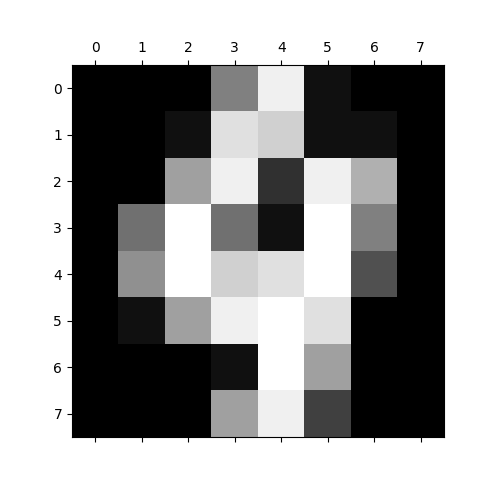
\includegraphics{mnist1.png}
show mnist

\section{baseline}
early stopping committee of nn 
bnn show better predictive performance 
though single early stopping sometimes perform at about the same predictive performance inconsistent across seeds 
cannot be explained away by 
\section{gnuts v xhmc}
xhmc better min ess 
variable num transitions after warmup
\section{gibbs v joint}
cp vs ncp 
observed multimodaility in sigma2 parameter 
nuts can sample hyperparameter well tho does not improve prediction

\section{sghmc}
impossible to tune , does not perform well
\section{scaled priors}
worse performance 
\section{adapt cov}
compare adapt cov. problem with inverting mass matrix
\section{num layers}
sampling about equally well across num layers
\section{float v double}
about same performance describes experiment 
stability 
test error 
can't talk about Rhat because multiple modes 
\section{HMC v NUTS}
better sampling performance by nuts >> better prediction 
\section{waic}
fails to predict best number of units . maybe bad mixing . talk about loo. psis
\section{sparsity inducing priors}
none of them predicts as well as normal prior 
horsehose type maybe  due to poor mixing 
but even gaussian inv gamma don't seem to do so well either

\section{Conclusion}
\chapter{Conclusion}
use xhmc, unscaled normal prior, 
use diag e 
don't use sghmc
don't use waic 
can use float on gpu

\chapter{Model}

\section{Markov Chain Monte Carlo}




\cite{green2015bayesian} gives a good summary of dynamical MCMC methods (langevin diffusion,MALA,HMC) and related convergence assessment methodologies.

In the late 80s and throughout the 90s, Bayesian statistical modeling became
feasible for a much larger class of problems than previously thought possible,
because of the availability of abundant computing power. Much work was produced
in MCMC methodologies\cite{robert2013monte}, theory\cite{tierney1994markov,roberts2004general} as well as in applications thereof.  



See more about Bayesian data analysis in \cite{gelman2014bayesian}. 


Evaluate sample quality
Effective sample size is defined as 
\[ ESS = N \{ 1 + 2 \sum_k \gamma(k) \}^{-1}, \]

estimated by the initial
monotone sequence estimator \cite{geyer1992practical}

It is a useful metric for measuring quality of the samples obtained from a
Markov Chain. We can take the mean or minimum ESS across all covariates.

Convergence diagnostics for high-dimensional target distributions. Theoretically, need convergence of the Markov Chain to the joint distribution, in practice only convergence to marginal distributions are checked. The literature has only looked at applying univariate diagnostics to each parameter individually and then calculate some summary statistic (mean,min) or carry out multiple testing if the diagnostic is based on a hypothesis test.

KL-divergence can be used to compare samples drawn from two different samplers.
The method advanced in \cite{boltz2007knn,boltz2007high} uses a kernel estimator to estimate the KL divergence between two empiricial distributions. The curse of dimensionality makes it difficult for application to high-dimensional posterior distributions $p(\theta|x)$, however, we can apply it to marginal predictive distributions $p(y|D)$ which usually are low-dimensional, when the covariates $x$ are fixed.

Tune MCMC algorithms. MCMC algorithms usually have a small number of tuning
parameters, such as a stepsize $\epsilon$, the number of leapfrog steps, or more
basic quantities like the length of the chain. Classic Bayesian methodology
\cite{robert2013monte} uses a mix of visual inspection of trace plots and
numerical convergence diagnostics like ESS as discussed earlier. The process
requires human intervention each time an algorithm is run and tuning parameters
readjusted after the diagnostics are computed. 


\section{ Hamiltonian Monte Carlo }. 

Originally developed in the physics community \cite{duane1987hybrid},
Hamilotnian Monte Carlo was introduced to the statistics community by Neal
\cite{neal2012bayesian}, 
by way of Computer Science, through his work on inference for Bayesian neural
networks. It was shown to be very efficient in sampling from high-dimensional
distributions and was used in the framework of bayesian inference to achieve superior predictive
performance in machine learning tasks\cite{guyon2004result}. However, its sensitivity to tuning parameters, relative difficulty of
implementation, and a lack of accessible
exposition to its theory, itself a subject of open research, precludes
widespread adoption. While some of these challenges remain to this day, the development of STAN \cite{carpenter2016stan} has made it significantly easier to carry out Bayesian inference with HMC, and is the main reason for increasing adoption of HMC in applications (cite statistics). Meanwhile, the invention Riemmanian Manifold Hamiltonian Monte Carlo (RMHMC) \cite{girolami2011riemann}, which exploits differential geometry to aid in local adaptation of the HMC sampler, and subsequent exploration the ideas introducd in the their paper, lead to better understanding of the mathematics behind HMC \cite{livingstone2016geometric,betancourt2014geometric} and  improvements to the sampler \cite{betancourt2013generalizing,betancourt2013general}. Many of these new developments have been and will be included in the STAN language. STAN also eliminates the need for tuning HMC. Users of STAN are shielded from the implementation details and tuning parameters settings, required only to specifiy the distributions involved in the models. 

Since STAN is so central to the present HMC literature, we would explain how it functions in the following exposition. Before that, however, we would explain the basic version of HMC on which STAN is built and to which many extensions are added. 












Now, STAN has many tiny yet crucial tricks which form part of the adaptive
tuning and diagnostic mechanism. Bear in mind that Bayesian inference with STAN is not completely
automatic because judgement still has to be made upon reviewing the results of
the returned samples to determine if they are valid. And like traditional MCMC
diagnostics this judgement is not completely objective in the sense that there
are no metrics that come with theoretical guarantees. 





Another problem with the above approach is that it is only unsuitable when the
target distribution can be approximately linearly transformed into a
distribution which can be easily explored by a standard HMC sampler.If the target
distribution has more complicated geometry that might differ in
curvature in various parts of its support, a constant $M$ is not enough to ensure
effective decorrelation during sampling. This motivates the use of
a location-dependent mass matrix $M(x)$ and is called the Riemannian Hamiltonian
Monte Carlo. More on this later. 






Note to preserve the correct invariant distribution, the calculation of the
potential energy function in the Hastings ratio must be done exactly. In later
discussion of stochastic gradient HMC sampler and extensions, we see data
subsamlping being combined with stochastic optimization to yield 
randomly varying the trajectory length is a recommended part of standard HMC
methodology. 

HMC is invariant to rotation.
Randomly choose stepsize. 
Shortcut method.
Mapping Multivariate Gaussian distribution. width of the distribution in the most constrained direction. Square root of the smallest eigenvalue of the covariance matrix for q.
Quote: HMC is valid as long as the dynamics is simulated using a method thatis reversible and volume-preserving. 

Tuning the HMC is tricky: for optimal stepsize see \cite{beskos2013optimal}

Understanding of optimal HMC stepsize, number of leapfrogs steps, number of leapfrog steps to reach nearly independent points.
Ex: Grows as $O(d^{1/4})$.







Symplectic  = volume-preserving


\section{Neural networks} 



\section{MCMC methods applied to hierarchical models}
\begin{enumerate}
\item Centered vs uncentered parametrization in hierarchical models.







\section{approximate inference for fast training and prediction}


Finally, there is the simple idea of approximating the the posterior
distribution by fitting a gaussian density around the posterior mode, this is
known as Laplace's method. It is first applied to BNNs by Mackay in \cite{mackay1992evidence}. In \cite{vivarelli2001comparing}, the author compared the predictive performance of Laplces's method against HMC and found the latter to perform slightly better, with more marked improvement on smaller datasets. An interesting point to note about this method is that by using a Gaussian approximation we have to calculate its covariance matrix by using the Hessian. Since neural network models are actually singular the Hessian is not positive definite everywhere and adjustments have to be made to make it work. In \cite{hernandez2015probabilistic} the authors compared Laplace's method with several approximate inference methods as well as HMC and found it to perform less well than the others. However, they constrained the covariance matrix of the Gaussian approximation to be diagonal to save computational time. Understandibly this leads to worse approximation. On the other hand, one is not forced to choose between a diagonal covariance or the full-rank one. Quasi-newton approximations are possible, and fits neatly within the optimization pipeline.

Variationa inference for bayesian neural networks started with the work of \cite{hinton1993keeping}, who developed a variational inference algorithm using the language of information theory. He used the concept of minimizing the description length of the weight, which is equivalent to minimizing the KL divergence as described above. 

Graves' work \cite{graves2011practical} built on the the Hinton's paper and introduced a stochastic gradient variational method. However, the stochastic gradient estimates are biased and the prior is limited to be Gaussian. In \cite{blundell2015weight} this is further improved upon using the re-parametrization trick \cite{opper2009variational,kingma2013auto,rezende2014stochastic}. This yields the Bayes by Backprops (BBB) algorithm.

The Expectation propogation (EP) approach to approximate inference in BNNs was experimented in \cite{jylanki2014expectation} but saw little follow-up because they method the authors developed was batch-only and could not scale to large datasets.A stochastic version was designed by \cite{hernandez2015probabilistic}, called the Probabilistic Backpropogation (PBP), and was shown to perform well on a wide range of test datasets. However, it has the limitation of being applicable only to regression problems. In \cite{ghosh2016assumed} it is extended to multiclass classification problems through a monte carlo approximation. 

In Myshkov et al's submission to a NIPS workshop (cite), the authors analyzed the performance of a few approximate inference algorithms for BNNs against the "gold-standard" that is the HMC, among those tested were PBP and EP. And they did not perform too poorly against MCMC methods. More analysis of this work to come later.  

In Bayesian dark knowlege, we also try to minimize the KL divergence, but do so
in a way that compresses model knowledge.  

Why do we assume the prior distribution of weight parameters to be normal centered at 0?

Study of prior distributions in neural networks.\cite{lampinen2001bayesian,titterington2004bayesian}

\section{Scaling MCMC methods to large datasets}




Expectation propogation. Original paper\cite{minka2001expectation}, Gelman and collegues wrote a paper on it \cite{gelman2014expectation}

Stochastic version discussed here \cite{li2015stochastic}
See also \cite{dehaene2015expectation} for another study of expectation propogation in the large sample size context. 

A stochastic natural gradient extension has been devised and applied to bayesian neural network models \cite{teh2015distributed}
Probabilistic Backpropogation is a special case of SEP applied to Bayesian neural networks \cite{hernandez2015probabilistic}.


Laplace Approximation. It is based on the second order approximation of the
log-likelihood of the posterior density around its mode.

Suppose the log posterior density $f(x)$ has a mode at $x^*$, then near $x^*$ we
have 
\[ f(x) = f(x^*) + \nabla f(x)|_{x=x^*} (x-x^*) + \frac{1}{2} (x-x^*)^TH(x-x^*)
\]
where $H$ is the Hessian matrix of $f(x)$ evaluated at $f(x)$, that is,
\[ H_{ij} = \frac{\partial^2 f(x)}{\partial x_i \partial x_j }|_{x=x^*} \]




\section{Bayesian Model Selection and Prediction}


\section{Multiple Modes}

Neural network models are known to have multiple modes, although it is widely believed that most local modes have similar likelihood values to the global mode. In Neal's work on bayesian neural network, he also assumed that multimodality would not cause any problems in inference and in prediction. 


Insert pseudocode. 
\chapter{Experimeints}
Plan:
Collect problems on which to fit neural networks of modest size. 

Example 1: Mackay's robot arm's data. 

This is a regression problem where the data is generated as follows:
\[ y_1 = 2.0 * \cos(x_1) + 1.3 \cos(x_1+x_2) + z_1 \]
\[ y_2 = 2.0 * \sin(x_1) + 1.3 \sin(x_1+x_2) + z_2 \]
where $z_1,z_2$ are independent Gaussian random variables of standard deviation
$0.05$ and $x_1$ is uniformly generated from $[-1.932,-0.453]\cup
[0.453,1.932]$, and $x_2$ is uniformly generated from the range $[0.534,3.142]$.
200 training cases and 200 test cases were generated according to the equations
above. 

A neural network with a single hidden-layer of 16 hidden units was used to model
the data.

Bayesian logistic regression with hierarchical prior. Following \cite{zhang2014semi}

1. Sample weights with HMC, sample hyperparameter with Gibbs sampling.

2. Same as above with Windowed update.

3. Same as 1 but with tempering. 

4. Sample weights and hyperparameter together with HMC. (STAN)

5. Softabs 

6. Empirical fisher information matrix 
Compare ESS/L.
Data: Same classification problem datasets from the RHMC paper \cite{girolami2011riemann}, as well as simulated data.
Funnel problem
Compare ESS/L as well as marginal distribution of the hyperparameter, which is known in this case. 

Bayesian neural network of more than 2 hidden units and of 1 hidden layer only. Test 1 layer network of 100 units with fixed normal prior and hierarchical prior.
Data: Same regression problem datasets from the PBP paper \cite{hernandez2015probabilistic}. 


For all the above problems it is straight forward to adapt code to compare manual hyperaparameter tuning with automatic tuning by STAN and by bayesian optimization. Compare ESS/L results for the final parameters selected. 

Test robustness of consensus mcmc to poor mixing. Split data into a $K$ subsets randomly, $K$ being a manageable small number (5 or 8), then tune some posterior distribution samplers to mix well and some others don't. Test on both regular and singular models.
 
For neural networks being used to fit a small number of observations relative to its dimension, there is a problem of overfitting. In \cite{gal2015bayesian}, it was shown that approximate bayesian inference via dropout helps to mitigate this problem. We argue that MCMC sampling would achieve even better performance.

Use only a small percentage (5 or 10 percent) of the MNIST dataset and perform batch inference with BNN. Try both fixed prior and hierarchical priors. Use the best sampler found from earlier experiments. 
Compare with gradient descent and dropout. 

Done with MCMC
Bayesian model selection. 
Bayesian neural networks can also be used to model data when the size of the training set is small. In this setting frequentist training of neural networks suffers from overfitting. Practioners who use neural network would like to make predictions for new data $\{x_{new}\}$. In principle, before making predictions the practioner should first decide on the model(s) to be used to fit the training data. While bayesian model averaging (BMA) is an interesting idea which promises to improve prediction accuracy, assignign prior to different models is difficult to justify and may appear arbritary. More importantly, for large models the time and memory complexity required to sample from the posterior distribution or the variational approximation thereof, as well as sample from the predictive distribution, would quickly become unmanageable as the number of models increases. 

For this reason, model selection is usually carried out, where a model is selected and then trained to make predictions on new data. Because there are infinitely many combinations of different tuning parameters and model structure paramters, an exhaustive search is impossible and instead a heuristic combinations of tuning paramters are chosen to form the candidtate models. Usually a holdout set (test set) is used to estimate the predictive performance of the model on new data. The model with the lowest average predictive error is then chosen. 

In bayesian statistics \cite{gelman2014bayesian} cross-validation, especially leave-one-out cross-validatino is recommended for model selection. It comes with a high computational cost, but remains the most principally sound method for estimating the out-of-sample log predictive density. WAIC(Widely applicable information criterion) is derived using singularity learning theory and estimates consistently the loocv, even for singular models. Traditional information criteria like AIC, BIC and DIC relies on the the asymptotic normality of the mle, which only holds if the Fisher information matrix is non-singular at the mle. While the justification of WAIC relies on heavy algebraic machinery, to apply it only requires being able to draw samples from the posterior distribution under a model and evaluate the likelihood.  
In the machine learning/deep learning community, model selection is usually done
by comparing the predictive accuracies of the different trained models on a
holdout set. The usual justification of this practice is that if the dataset
exhibits enough data redundancy then  this is enough to estimate the test
accuracy. However, this is certainly dependent on the particular dataset and the
size of the model one would like to use to fit the data. The most statistically
principled practice would be too use all available data to train models and then
select the best model using cross-validation. Efficeint approximation to the
cross-validation log density like the WAIC is therefore deemed desirable for
model selection. 

An important statistical question is therefore as follows: for neural network models, is
the use of a holdout set for model selection consistent with best practice?
That is, do these two methods make the same model selection decision ? What happens
in the small data regime? I suspect the utitilty of WAIC would be the greatest
in small-to-medium data size settings, where a randomly chosen subset that is 25
percent the size of total dataset is unlikely to estimate the test error with a
low variance (unbiased by highly variable).

Approximation inference. 
Compare PBP, BBB, LA, to HMC and SGD. Use fixed prior. Test effect of small training
set. Compare time to reach test accuracy. Use importance sampling to calculate
WAIC. Decrease memory until these approximation methods perform better than
MCMC.

Scaling MCMC
SGLD, SGHMC, pSGLD, SGFS, Thermostat. Compare test accuracy with batch HMC.
Tuning by test accuracy, or tuning by ESJD.

Consensus MCMC 
See if singularity severely degrades quality of classification.

Effects of pruning
In the BBB paper, performance does not degrade drastically even if 98 percent of
the weights are removed. See same thing applies to MCMC samples. 





But before all this can start we first need to overcome the difficulties of
sampling from the posterior distribution of a bayesian neural network. The
first source of difficulty comes from the correlation in the posterior distribution induced by
the connection between neurons in consecutive layers. Each neuron in a layer is
connected to all neurons from the previous layer and hence is influenced by
values in the previous layer. This is the first source of correlation. The
second source of correlation comes from the use of a hierarchical prior on the
weights of the network. This is tackled by Riemmanina Manifold type MCMC
methods, which make use of information of the second derivatives of the
log-posterior. The trade-off is now a linear system of full rank must be solved
to calculate each update in the markov chain. This has the time complexity of
$O(p^3)$ which makes it difficult to apply to neural network models, who's
expressiveness comes from its large number of parameters. 

Posterior correlation due to hierarchical prior vs inter-layer correlation. 

The second source of difficulty comes from the cost of evaluating the
log-posterior density and its derivative with respect to the parameters. For
exact calculation, both requires going through the entire dataset. In
frequentist fitting of neural networks, this problem is bypassed by evaluating
the gradient using a random subset of the original datapoints as input. The mcmc
analogues are stochastic gradient mcmc methods. These methods, however, suffer
from slow mixing in the case of SGLD variants, and the need to do matrix
inversion in the case of SGHMC variants. Interesting compromise can be made by
replacing the full fisher information matrix by a diagonal matrix or low-rank
approximations. 

And other obstacle prevents the widespread adoption of mcmc for inference in BNN
is the dependance on GPUs for calculating the gradient of the weights by
backpropogation. GPUs make fast calculation of gradient of networks with
increasing number of layers feasible, however its downside is its limited
fast-access memory. Transferring weights from the GPU to the main disk creates a
bottleneck in the calculation that balances out the speed gain. Even if we
disregard the problem with speed and only focuses on the memory, we find that
bayesian inference by mcmc as carried out traditionally by the statistics
community, where a large number of samples from the chain is generated and
saved, diagnosced for convergence and then quantities where expectation is taken
with respect to the posterior distribution are approximated by taking
expectation with respect to the empirical distribution instead. The first
problem with this approach is the lack of tool for assessing convergence for
high-dimensional distributions. Convergence of every marginal distribution does
not imply convergence of the joint distribution. Also, it is impossible to
visually inspect
the trace plot of all covariates along the chain in order to assess convergence,
depriving ourselves one of the more reliable tools in the classical mcmc
methodology. Another problem with the traditional methodology is the necessity
to compute a long chain (even after thinning) and use the samples for expectaion
calculation. No matter how decorrelated the samples from the chain are,
more than a handful of samples at a time is required to calculate an unbiased
estimate of the expectation that doesn't suffer from high variance. This limits
the size of the network that can be trained, often it precludes the use of a GPU
altogether and limit us to shallow networks. A frequentist training of neural
network only $O(p)$ memory is required to store the weights in memory, but in
the bayesian framework described above $O(pT)$ memory is required, where $T$ is
the number of samples from the chain that we wish to retain. In many
applications a large
model of 1 million paramters is found to minimize the test error on a holdout
set among many possible model structure. One might then wish to assign prior to
weights in this network and carry out bayesian inference. Even assuming there is
enough memory on the GPU, it is reasonable to assume that in most applications it might not be worth the 50 times increase in memory
budget to improve predictive accuracy by 2 percent. 

Since neural networks are 
mostly used for predictive purposes and there is little interpretability in the
posterior distribution of the individual weights, which are
always integrated out to find the predictive distribution anyway, one might find
it worthwhile to look at approximate inference methods that aim to find
an approximation to the posterior distribution with a tractable distribution and
which allows for easy calculation of the posterior predictive distribution. 

One note that to calculate the WAIC, the memory requirement is only $O(nT)$,
where $n$ is the number of observations and $T$ the number of mcmc samples. This
inspires the methdology of bayesian model selection and inference. First we
choose the model by using the most efficient mcmc methods. Since evaluation of
the WAIC is independent of the dimension of the model, this can be done on the
GPU and enjoy the speed up that it provides. Once the model is chosen,
approximation inference is carried out to fit an approximate model that allows
fast training and prediction, with most variations using $O(p)$ memory.

While batch version of HMC is not practical because of size constraints, for
research purposes or small data problem it might be necessary to simulate a
markov chain that is as targeting as close the posterior distribution as
possible, excluding stochastic gradient versions where bias is introduced by
dropping the metropolis correction step. A comparative study of the effectivenss the new
RMHMC type samplers applied to jointly sample the weights and hyperparameters is
long due. 

Make the connection between natural gradient learning and riemannian manifold
hmc



What is the largest neural networks that can be trained by modern hardware using 1996 techniques (HMC tuned by heuristics plus windowed state) from Neal's thesis?  

How good are the samples generated using these techniques? Look at min effective sample size across all covariates. Trace plot of randomly selected components/ hyperparameters. Should see skewed distribution. Plot it.


Train models of moderate size first (can fit on harddisk, most likely 1 hidden layer), then apply Riemman Hamiltonian Monte Carlo to see if you get much better results. Also compare that to just normal approximation around max. Multiple mode seems to be a problem. But also have result(heuristics) from frequentist results saying that local min is not a serious problem cuz most local modes are similar cost value. 

Sample using MALA, then Riemann MALA.

The langevin dynamics algorithm has fewer tuning parameters, but mixes slower. Hope is that Riemann MALA is a compromise between MALA and full HMC. 

Compare different metrics used in RHMC. 

How much does initialization matters. i.e. Initialize to random normal covariates vs variance-matching initialization. See Xavier initialization: 
\[X \sim U[- \sqrt{\frac{6}{n_{in}+n_{out}}}, \sqrt{\frac{6}{n_{in}+n_{out}}}] \]

Compare predictive accuracy reached under fixed time budget.

Simulation studies: 

Target distribution: multivariate student-t distribution. Zero mean and diagonal covariance with common variance. See Jake Baker's master's thesis.His simulations don't stress the samplers as much as I'd wish. For example the highest dimension tested was 20. 

He used the KL divergence as performance metric, calculated as follows \cite{boltz2007high}. 

Since we care about prediction, we can follow Mykshov by comparing different MCMC samplers/approximate bayesian inference using the KL divergence of the predictive distribution with the $x$ integrated out instead. First, this is usually a one dimensional distribution, which makes much more sense when we are using kernel methods to approximate the KL divergence anyway.

Funnel distribution: typical of bayesian models with hierarchical priors. Neal has used slice sampling and HMC to draw from it. Betancourt used Riemmanian HMC with his metric. 

Hasn't been done: MALA, RMALA, HMC with partial momentum, windowed,
semi-separable HMC (benchmark),RHMC with softabs(hasn't been a comparison of
ESS) adaptive HMC (Gaussian process) each of the HMC variety above can also be

coupled with the trick in \cite{burda2011bayesian} (fix conditioning matrix
between each sample).
Experiment with efficient diagonal approximation to covariance matrix.

Hierarchical bayesian logistic regression: Methods above as well as stochastic
gradient MCMC (sgld,pre-conditioned sgld, thermostat,sghmc)
Try on simulated data as well as benchmark datasets.


Bayesian dark knowledge: how does the quality of the MCMC samples from the
posterior distribution of the teacher model affect the approximation of the
prediction distribution by the student neural network. How sensitive is it?


Memory efficient implementation of MCMC.
Keep history of random seeds for mv normals, as well as history of acceptance
decision.
Given only $\theta_T$, can reproduce chain $\{\theta_1, \dots, \theta_T \}$ on
command.
Useful for GPU implementations of MCMC.
Predictive performance(cross-validation) used for adaptive
tuning\cite{wang2013adaptive}


Using predictive performance as metric to tune MCMC. i.e. select tuning
parameters that give the highest average posterior predictive density for new
data or highest accuracy on test set.

Compare variational posterior to true posterior.  

Statistical question: compare the train/test holdout metric to WAIC. Do they
give the same conclusions?\cite{kohavi1995study}
Try k-fold cross-validation as well.

Evaluate variational models in terms of WAIC. 

Work using evidence aka marginal likelihood for neural network model comparison. 
\section{ neural networks}
Previous work:\cite{blundell2015weight}

Suppose the dimension $p$ of $\theta$ is so high that we can only afford to keep 20 copies or so of $\theta$ in memory (on a GPU, for example). 
What is the best practice (MCMC vs variational inference) for bayesian inference in this scenario. 

Effect of number of layers on autocorrelation.(with or without hierarchical prior).

Model selection as follows: select certain quantities to monitor convergence (hyperparameters, acceptance ratio etc), store values needed to calculate WAIC, select model. Then use approximate inference (variational inference or expectation propogation) to compute approximation to predictive distribution for predictions.

Sgmcmc: how many minibatches of data should be used to update the main paramters before switching to sampling hyperparameters? In sghmc, they have examples where the entire dataset is passed through and the other just some data.
Goal: 

stochastic gradient quasi netwon langevin dynamics requires extra tuning paramters with little guidance on how to tune them \cite{csimcsekli2016stochastic}

preconditioned sgld introduces bias\cite{li2015preconditioned}.
\bibliographystyle{plain}

\end{enumerate}
\bibliography{test}
\end{document}
